\loop\iftrue%
\errmessage{This article is copyrighted and should not be TeXed}%
\repeat%
\documentclass{ifacconf}

\usepackage{graphicx}      % include this line if your document contains figures
\usepackage{natbib}        % required for bibliography
\usepackage[inline]{enumitem}        % required for bibliography


%\setlength{\textfloatsep}{1.2\baselineskip plus  0.2\baselineskip minus  0.4\baselineskip}

\usepackage[utf8]{inputenc}
\usepackage{graphicx}
\usepackage{xargs}
%\usepackage{pdfcomment}
\usepackage{tikz}
\usepackage{microtype}
\usepackage{siunitx}
\usepackage{longtable,tabularx}
\setlength\LTleft{0pt}

\usepackage[math]{blindtext}
\usepackage{xcolor}

\usepackage{import}
\usepackage{subcaption}
\usepackage{moreverb}

% \usepackage[bbgreekl]{mathbbol}
% \usepackage{mathbbol}
% \DeclareSymbolFontAlphabet{\mathbbl}{bbold}
\usepackage{graphicx}
\usepackage[many]{tcolorbox}

% \usepackage{physics}
% \usepackage{placeins}
\usepackage{float}
\usepackage{amsmath}
\usepackage{amssymb}
\usepackage{booktabs}
\usepackage[notextcomp]{stix}
\usepackage{mathtools}
%\DeclareSymbolFontAlphabet{\mathbb}{AMSb}
%\DeclareFontFamily{U}{stix2bb}{\skewchar\font127 }
%\DeclareFontShape{U}{stix2bb}{m}{n} {<-> stix2-mathbb}{}
% \DeclareMathAlphabet{\mathbb}{U}{stix2bb}{m}{n}

\usepackage[ddmmyyyy]{datetime}
\usepackage[linesnumbered,ruled,vlined,algo2e]{algorithm2e}

\newif\ifdebug%
\newcommand{\draft}{\debugtrue}
\newcommand{\final}{\debugfalse}
\newcommand{\todo}[2][FORGOT TO DO SOMETHING]{\ifdebug%
	{%
	  \color{red}
	  #2}\else \PackageError{}{#1}{#2}#2\fi}%
\newcommand\doing[2][FORGOT TO DO SOMETHING]{\ifdebug%
	{%
	  \color{blue}
	  #2}\else \PackageError{}{#1}{#2}#2\fi}%
\newcommand\warning[1]{\ifdebug%
	{%
	  \color{red}
	  #1}\fi}
\renewcommand\note[2][]{\ifdebug%
  {\pdfcomment[color=red,opacity=0.4,subject=note,author=#1]{#2}} \fi}
\newcommand\highlight[3][]{\ifdebug%
  {\pdfmarkupcomment[color=red,opacity=0.4,author=#1]{#2}{#3}} \fi}


\newcommand\lastcompiled{\footnotesize{\warning{Compiled on \today{} at \currenttime}}}

\newcommand{\mysmall}{\fontsize{7.5pt}{8pt}\selectfont}
\newcommand{\no}[1]{}

\usepackage{lineno}
%\usepackage{hyperref}
%
%% \AtBeginDocument{
%\hypersetup{
%   % pdfauthor   = {\@author},
%	 % pdfproducer = {LaTeX},
%   % pdftitle    = {\@title},
%   % pdfkeywords    = {\@keywordsEN},
%   % pdfsubject = {\@subject},
%   colorlinks=true,
% }
% }


%\modulolinenumbers[5]
% Each section on new page?
% \newcommand{\jsection}[1]{\clearpage \section{#1}}

\graphicspath{{../img/}}


\newcommand{\N}{\mathbb{N}}
\newcommand{\Z}{\mathbb{Z}}
\newcommand{\Q}{\mathbb{Q}}
\newcommand{\R}{\mathbb{R}}
\newcommand{\C}{\mathbb{C}}
\newcommand{\T}{^{\mathrm{T}}}
\newcommand{\1}{\mathbf{1}}
\newcommand{\0}{\mathbf{0}}

\newcommand{\unitInterval}{\set{E}}

\newcommand{\abs}[1]{\left\lvert#1\right\rvert}
\newcommand{\norm}[1]{\lVert#1\rVert}
\newcommand{\ubound}[1]{\overline{#1}}
\newcommand{\lbound}[1]{\underline{#1}}
\newcommand{\pre}[1]{\overleftarrow{#1}}
\newcommand{\post}[1]{\overrightarrow{#1}}
\newcommand{\upd}[1]{{#1}^\prime}

\newcommand{\blkdiag}{\mathop{\rotatebox{90}{$\diameter$}}}
\newcommand{\dir}{\mathop{dir}}
\newcommand{\until}{\mathbin{:}}
\newcommand{\setbuild}[2]{\{#1\mid#2\}}
\newcommand{\seq}[2][n]{\lbrace #2_{0},\ldots,\,#2_{#1} \rbrace}
\newcommand{\hadamard}[2]{#1\circ #2}
\newcommand{\kron}[2]{#1\otimes#2}
\newcommand{\symmetric}{\mathbb{S}}
\newcommand{\semidefpos}{\mathbb{S}_{+}}
\newcommand{\defpos}{\mathbb{S}_{++}}
\newcommand{\elem}[2][1]{{#2}_{(#1)}}
\renewcommand{\implies}{\Rightarrow}
\renewcommand{\iff}{\Leftrightarrow}
\newcommand{\argmax}{\mathop{\arg\!\max}}
\newcommand{\argmin}{\mathop{\arg\!\min}}
\newcommand{\maximize}{\mathop{\textrm{maximize}}}
\newcommand{\minimize}{\mathop{\textrm{minimize}}}


\newcommand{\inspacey}[0]{\; \in \,}
\newcommand{\mbf}[1]{\mathbf{#1}}
\newcommand{\mbb}[1]{\mathbb{#1}}
\newcommand{\apriori}[0]{\textit{prior}}
\newcommand{\Apriori}[0]{\textit{Prior}}
\newcommand{\aposteriori}[0]{\textit{posterior}}
\newcommand{\Aposteriori}[0]{\textit{Posterior}}
% \newcommand{\final}[0]{\textit{ final }}
% \newcommand{\Final}[0]{\textit{ Final }}

\newcommand{\minksum}[0]{{\mbox{\scriptsize $\bigoplus$}}}
\newcommand\at[2]{\left.#1\right|_{#2}}
\newcommand{\imid}[1]{\operatorname{mid}(#1)}
\newcommand{\rad}[1]{\operatorname{rad}(#1)}
\newcommand{\RM}[2]{{\ensuremath{\mbf{R_{\mathrm{#1 #2}}}}}}
\newcommand{\Matlabbrand}{Matlab\textsuperscript{\tiny{\textregistered}}\;}
\newcommand{\dotp}[2]{\langle #1,#2\rangle}
\newcommand{\pdv}[2]{\frac{\partial #1}{\partial #2}}
\newcommand{\smallfigwidth}{0.99\linewidth}
%\newcommand{\cz}{\ensuremath{\mathcal{C}\mathrm{-zonotope}}}
%\newcommand{\czs}{\ensuremath{\mathcal{C}\mathrm{-zonotopes}}}
\newcommand{\pluseq}{\mathrel{+}=}
\newcommand{\set}[1]{\mathcal{#1}}
\renewcommand{\vec}[1]{\boldsymbol{#1}}

\usepackage[acronym]{glossaries-extra}%
\setabbreviationstyle[acronym]{long-short}

\newcommandx\acr[5][4=,5=]{
  \ifthenelse{\equal{#5}{}}
  {
    \acrSing{#1}{#2}{#3}
  }
  {
    \acrPl{#1}{#2}{#3}{#4}{#5}
  }
  \expandafter\newcommand\csname #1long\endcsname{\glsdesc{#1}}
  \expandafter\newcommand\csname #1short\endcsname{\glsname{#1}}
}

\newcommandx\symbl[4][4=,]{
  \ifthenelse{\equal{#4}{}}
  {
    \symblnosort{#1}{#2}{#3}
  }
  {
    \symblwithsort{#1}{#2}{#3}{#4}
  }
}

\newcommand{\acrSing}[3]{\newacronym{#1}{#2}{#3}
  \expandafter\newcommand\csname #1\endcsname{\gls{#1}}}

\newcommand{\acrPl}[5]{
  \newacronym[plural=#4,firstplural=#5 (#4)]{#1}{#2}{#3}
  \expandafter\newcommand\csname #1\endcsname{\gls{#1}}
  \expandafter\newcommand\csname #1s\endcsname{\glspl{#1}}
}

\acr{vtwox}{V2X}{Vehicle to everything}
\acr{uwb}{UWBR}{Ultra-Wideband Ranging}
\acr{gnss}{GNSS}{Global Navigation Satellite Systems}
\acr{rtk}{RTK}{Real Time Kinematics}
\acr{kf}{KF}{Kalman Filter}
\acr{linearinclusion}{LI}{linear inclusion}[LIs][linearinclusions]
\acr{ekf}{EKF}{Extended Kalman Filter}
\acr{ukf}{UKF}{Unscented Kalman Filter}
\acr{sivia}{SIVIA}{Set Inversion Via Interval Analysis Algorithm}
\acr{vsivia}{VSIVIA}{Vectorized SIVIA}
\acr{zoh}{ZOH}{Zero-Order Hold}

\acr{smf}{SMF}{Set Membership Filter}[SMFs][Set Membership Filters]
\acr{czesmf}{CZESMF}{Constrained Zonotope Extended Set Membership Filter}
\acr{iesmf}{IESMF}{Iterated Extended Set Membership Filter}
\acr{ia}{IA}{Interval Arithmetic}
\acr{tddd}{T3D}{Time-Differenced Double phase Difference}
\acr{uas}{UAS}{Unmanned Aircraft System}[UASs][Unmanned Aircraft Systems]
\acr{cz}{$\mathcal{CZ}$}{Constrained Zonotope}[$\mathcal{CZ}$s][Constrained Zonotopes]
\acr{cgrep}{CG-Rep}{Constrained Generator Representation}
\acr{grep}{G-Rep}{Generator Representation}
\acr{hrep}{H-Rep}{Half-space Representation}

\glsdisablehyper


\newtheorem{remark}{Remark}
\def\th@remark{%
    \thm@headfont{\itshape}%
    \normalfont % body font
    \thm@preskip\parskip \divide\thm@preskip\tw@
    \thm@postskip\z@
  }


\GlsXtrEnableEntryCounting
 {acronym}% list of categories to use entry counting
 {1}% trigger value

\draft
% \journal{Control Engineering Practice}
%\usepackage[top=57pt, left=48pt, right=48pt, bottom=43pt]{geometry}

%===============================================================================
\begin{document}
\begin{frontmatter}


\title{Guaranteed autonomous vehicles localization under uncertain observation times using constrained zonotopes set-membership filtering} 
% Title, preferably not more than 10 words.

%\thanks[footnoteinfo]{Sponsor and financial support acknowledgment
%goes here. Paper titles should be written in uppercase and lowercase
%letters, not all uppercase.}

\author[First]{Rafael Accácio Nogueira} 
\author[Second]{Soheib Fergani} 
%\author[Third]{Third C. Author}

\address[First]{Univ Angers, LARIS, SFR MATHSTIC, {F-49000 Angers, France}  (e-mail:~rafael-accacio.nogueira@univ-angers.fr)}
\address[Second]{Université de Toulouse, LAAS-CNRS, Toulouse, France (e-mail:~sfergani@laas.fr)}
%\address[Third]{Electrical Engineering Department, 
  % Seoul National University, Seoul, Korea, (e-mail: author@snu.ac.kr)}
\begin{abstract}                % Abstract of 50--100 words
  This paper presents a set-based state estimator using constrained zonotopes for nonlinear systems with uncertain and asynchronous observation times.
  This estimator also accounts for parametric uncertainty in the observation equation and allows multiple state propagation models to be combined. The method provides guaranteed state enclosures despite observation time uncertainty, which is critical in practical autonomous vehicle applications. Its effectiveness is illustrated on two academic case studies representative of real-world scenarios: a one-dimensional vehicle platooning problem and a two-dimensional vehicle localization problem. The filter is compared against other methods highlighting its performance.
  % an ellipsoidal set-based estimator (IESMF), a vectorized implementation of the nonlinear set inversion algorithm SIVIA, and the classical Extended Kalman Filter (EKF), highlighting both its robustness and performance.
\end{abstract}
%\begin{abstract}                % Abstract of 50--100 words
%  This paper presents a set-membership state estimator based on constrained zonotopes, addressing uncertain asynchronous observation times.
%  Additionally, the proposed estimator accounts for parametric uncertainty in the observation equation and incorporates multiple state propagation models.
%  The filter provides valid state enclosures despite observation time uncertainty, which is critical for real-world applications.\\
%  To demonstrate its effectiveness, we present academic problems simulating real-world applications (vehicle platooning and vehicle ).
 % Comparisons with existing nonlinear estimation algorithms, including the ellipsoidal set state estimator (IESMF), the set inversion algorithm (SIVIA), and the classic Extended Kalman Filter (EKF), highlight its efficiency and performance improvements of the proposed approach.

%\end{abstract}

\begin{keyword}
  
 Set-membership estimation,
  Constrained zonotopes,
  Asynchronous observations,
  Uncertain sampling times,
  Nonlinear systems,
  Robust sensor fusion,
  Autonomous vehicles localization,
\end{keyword}

\end{frontmatter}
%===============================================================================
\section{Introduction}

Over the last decade, autonomous vehicles have significantly increased their autonomy and integration into everyday life. Vehicle platooning and tight formations may require cooperative estimation of relative positions and velocities with high accuracy in order to guarantee safety and efficiency, such as studied in \cite{meng2021v2v} and \cite{gao2022performance} using \vtwoxshort\ and \uwbshort.
%Over the last decade, unmanned and autonomous vehicles have significantly increased their level of autonomy and their integration into everyday life, notably through autonomous cars and mobile robots. Cooperation among such agents enables configurations such as vehicle platooning and tight formations. These configurations require relative positions and velocities to be estimated with high accuracy, often at the decimeter level or better, in order to guarantee safety and efficiency.
%For instance, recent studies have explored robust cooperative localization for connected vehicles using \vtwox\ and \uwb\  (\cite{meng2021v2v} and \cite{gao2022performance}).


In practical implementations, nonlinear process and observation models make state estimation challenging. Techniques such as the \ekf{} are widely used due to their relatively low computational cost and ease of implementation.
However, these methods rely on assumptions on the probability distributions of process and observation noises that may be violated in practice.
Moreover, they provide no formal guarantees that the true state lies within prescribed confidence regions.

\smfs\ offer an alternative framework where uncertainties are described by sets, thus, no assumptions on error distributions are made and state estimation computes sets containing the state.
However, nonlinear set computations may be intractable, what motivated practical algorithms relying on over-approximations using simpler sets such as ellipsoids~\citep{Bolting2018b}, and intervals~\citep{RohouJaulin2021}.

Subpaving approaches, such as \sivia, were used in~\cite{bonnifait2017cooperative} to localize vehicles, providing tight enclosures in nonlinear state estimation.
However, for such methods, computation time usually grows exponentially w.r.t. the dimension of the state, limiting their real-time applicability to higher-dimensional system.
% Overall, the main challenge is the trade-off conservatism vs. computational effort.
%Despite their accuracy, the computation time of such methods typically grows exponentially with the dimension of the state, limiting their real-time applicability to higher-dimensional systems. Overall, the main challenge is the trade-off conservatism vs. computational effort.

%Applications of \smf\ state estimation in autonomous vehicles settings have been recently address, e.g., vehicle platooning and urban navigation had been treated using interval formalism for guaranteed localization in \cite{ gning2006constraints} and \cite{guyonneau2014guaranteed}, and  ellipsoidal or set-membership fusion for GNSS/\uwb-based navigation in \cite{yu2016ellipsoid}. 

In~\cite{scott2016constrained}, \czs{} have been proposed as a new set representation.
\czs\ incorporate constraints to zonotopes, allowing one to represent general convex polytopes while retaining efficient computation of key operations.
A first application to nonlinear systems appeared in \cite{rego2018set}, where observations were assumed linear in the states.% and in \cite{wang2024data}, to autonomous vehicle localization.

In 2019, the core idea of the algorithm presented in this work was patented in Europe~\citep{patent_CZESMF}.
The proposed method uses linearization to propagate state predictions. %, in contrast to \cite{rego2018set}, where interval bundles are used for propagation.
Later, \cite{RegoEtAl2020} adopted similar strategies and introduced mean-value extensions; subsequent contributions included consistency checks through invariants~\citep{RegoEtAl2021},
efficient nonlinear uncertainty propagation %using \cz\ formulations
\citep{facerias2024distributed} and new volume-reduction techniques~\citep{rego2025novel}.

% \czs\ have also been used in reachability analysis~\citep{YangEtAl2022b} and in studies on the complexity of set operations~\citep{AlthoffEtAl2021}.

However, to the best of the authors' knowledge, none of these works explicitly address the problem of uncertain observation times and existing approaches typically assume synchronized measurements. 
In many applications, sensor timestamps may be affected by jitter, delays or synchronization issues, which may degrade estimation performance, if not accounted for.

This article address this gap by extending a \cz-based \smf\ to handle uncertain observation times. The main contributions are:
\begin{itemize}
  \item An easily implementable \smf\ for nonlinear systems based on constrained zonotopes admitting asynchronous observations with uncertain observation times.% by explicitly inflating observation intervals to account for timing uncertainty.
  \item A benchmark study comparing the proposed filter with \iesmfshort~\citep{Bolting2018b}, \vsivialong\ \citep{herrero2012efficient}, and the traditional \ekf.
\end{itemize}

The paper is organized as follows.
Section~\ref{sec:preliminaries} recalls the necessary background on set-membership.
In Section~\ref{sec:problemstatement}, we formulate the set-based estimation problem and introduce the system and observation models.
Section~\ref{sec:zesmf} presents the filter.
In Section~\ref{sec:examples} we show implementation details and numerical results for two examples where we compare the proposed filter with other algorithms. Finally, future directions are provided in Section~\ref{sec:conclusion}.
%
%\section{Introduction}
%% General Context
%Over the last years, unmanned vehicles have seen a considerable rise in their level of autonomy, and as a consequence their integration on general public's use, notably autonomous cars.
%% Pros of Cooperation for formation
%Cooperation among those agents yields configurations such as platooning and tight formations, which require
%relative positions of vehicles need to be estimated with decimeter level, if not centimeter level accuracy.%~\cite{Bolting2016}.
%
%Due to nonlinearities, in practical implementations, techniques such as the \ekf{} are widely used.
%However, as it is known, many of them violate the underlying assumptions of knowledge of the distributions of both process and observation model's uncertainties~\citep{simon2006optimal}.
%
%
%\smfs\ offer an alternative:
%no assumptions about error distributions are required.
%Nonetheless, exact estimation may be intractable for nonlinear systems.
%Recently, algorithms have been proposed, employing over-approximations of simpler sets such as ellipsoids~\citep{MerhyEtAl2020}, intervals~\citep{RohouJaulin2021}, zonotopes~\citep{WangEtAl2018} and collections thereof~\citep{AlthoffKrogh2011}.
%
%
%
%Subpaving approaches, such as the \sivia, were used in~\cite{bonnifait2017cooperative} to locate  ground vehicles providing tight enclosures for nonlinear state estimation.
%Regardless the tight enclosures, since the computation time increases exponentially with respect to the number of dimensions used, this fact restricts its usefulness for multiple dimensions and real-time applications.
%The common challenge for all \smfs\ is finding the trade-off between conservatism and computational effort.
%
%
%The recently proposed \czs{} \citep{scott2016constrained} are an alternative to deal with this challenge.
%A \cz{} expands the definition of zonotopes by integrating linear constraints.% representing any convex polytope with lower computational effort to execute some operations.
%
% As additional advantage, \czs\ are closed under intersection, seeming promising compared to existing linear set state estimators, as reported in \cite{scott2016constrained}, where randomly generated linear systems have been considered.
%
%A first application to nonlinear systems appeared in \cite{rego2018set}, where observations were assumed to be linear in the state. % and no observation time uncertainty is considered.
%In 2019, the base of the algorithm we present in this work was patented in Europe~\citep{patent_CZESMF}. %\footnote{U.S. patent pending .}.
%This algorithm employs linearization to directly propagate the state predictions, differently of \cite{rego2018set}, where
%the authors use interval bundles to propagate the set.
%Later works, such as~\cite{RegoEtAl2020}, used similar linearization strategy and presented another approach through mean value extension.
%After that, authors included consistence check through invariants~\citep{RegoEtAl2021} and volume reduction through the use of difference of convex functions~\citep{PaulaEtAl2024}.
%Other works used \czs\ for backward reachability analysis~\citep{YangEtAl2022b} and compared on the complexity of operations on different sets~\citep{AlthoffEtAl2021}.
%
%However, as far as we are concerned, none of them took interest on uncertain observation times. Thus, in this article, the main contributions are the following:
%\begin{itemize}
 % \item
  %      An easily implementable \smf\ for nonlinear systems based on constrained zonotopes that admits asynchronous observations with uncertain observation times.
  %\item A benchmark example, comparing it performance-wise with the ellipsoidal set-based \iesmf~\citep{Bolting2018b}, as well as a vectorized implementation of the less conservative nonlinear set inversion algorithm \sivia\ \citep{herrero2012efficient} and the traditional \ekf.
%\end{itemize}
%
%The article is structured as follows:
%We lay in Section~\ref{sec:preliminaries} the mathematical background.
%In Section~\ref{sec:problemstatement}, we pose the set-based estimation problem.
%Then, in Section~\ref{sec:zesmf} we present the \cz-based \smf.
%Section~\ref{sec:examples} illustrates the implementation steps in two localization problems and compare filter performance with other algorithms.
%Finally, in Section~\ref{sec:conclusion}, through some remarks on results, future work is delimited.
%
%
\section{Preliminaries}\label{sec:preliminaries}
\vspace{-0.2cm}
\subsubsection*{Notation}~\\
${[M]}$, $[\vec{v}]$ and $[a]$ denote interval matrices, vectors and scalars, with lower and upper bounds ${\smash{\lbound{\square}}, \smash{\ubound{\square}} \in \R^{m \times n}}$, e.g.  $[a]=[\lbound{a}, \ubound{a}]$.
We denote ${\unitInterval=[-1,1]}$.
$\imid{[M]}$ and $\rad{[M]}$ are the mid and radius of interval $[M]$.
The reader is referred to \cite{jaulin2001applied} for other concepts.
To accommodate for heterogeneous sampling times, we adopt the notation $\vec{x}(t_l)$, where $t_l$ indicates the time of validity of $\vec{x}$.
% The discrete nature of filter execution is captured by indexing the time.
Similarly, $\set{Z}(t_k)$ indicates the set is valid at the time $t_k$, i.e., ${\vec{x}(t) \in {\set{Z}}(t_k)}$ if ${t=t_k}$.
An interval $[t_k]$ indicates validity for all times in this interval, i.e., ${\vec{x}(t) \in \set{Z}([t_k])}$ ${\forall t \in [t_k]}$.
% This concept becomes important when dealing with uncertain observation times.
A \Apriori\ (\aposteriori) set is
denoted $\smash{\pre{\square}}$ ($\smash{\post{\square}}$).
When unambiguous, indexed variables correspond to sets of the same index, e.g., ${\set{Z}_a = \langle G_a,\vec{c}_a,A_a,\vec{b}_a\rangle}$.
The gradient of $\vec{g}(\vec{a},\vec{b})$ w.r.t.\ $\vec{a}$ evaluated at ${(\bar{\vec{a}},\bar{\vec{b}})}$ is $\vec{g}_{\vec{a}}(\bar{\vec{a}},\bar{\vec{b}})$.
The direction of $\vec{x}$ is $\dir(\vec{x})=\vec{x}\norm{\vec{x}}^{-1}$.

\subsection{Constrained Zonotopes}
\vspace{-0.2cm}
As proposed in~\cite{scott2016constrained}, given ${G\in \R^{n\times m}}$, ${\vec{c}\in \R^n}$, ${A\in\R^{c\times m}}$ and ${\vec{b}\in\R^{c}}$, a \cz\ is represented as
\begin{equation}
  \set{Z}= \langle G,\vec{c},A,\vec{b}\rangle = \{G \vec{\xi} + \vec{c} \; \mid \; \norm{\vec{\xi}}_\infty \leq 1, A\vec{\xi} = \vec{b}\}  \subset \mathbb{R}^n.
\end{equation}
$[\set{Z}]$ is its interval hull and
$\set{Z}([\vec{a}])$ the \cz\ representation of $[\vec{a}]$.

Given three \czs, ${\set{Z}_a\subset\R^{n}}$, ${\set{Z}_b\subset\R^{n}}$ and ${\set{Z}_c \subset \R^k}$, and a matrix ${R\in\R^{k\times n}}$,
the operations over \czs\ are given by:
\begin{align}
  R\set{Z}_a=&\langle RG_a,R\vec{c}_a, A_a,\vec{b}_a\rangle,\\
  \set{Z}_a + \set{Z}_b=&\left\langle
                          \left[\begin{smallmatrix}
                            G_a&
                                 G_b
                          \end{smallmatrix}\right] ,\vec{c}_a+\vec{c}_b, \left[\begin{smallmatrix}
                            A_a& 0\\
                            0  & A_b
                          \end{smallmatrix}\right],
                          \left[\begin{smallmatrix}
                            \vec{b}_a\\
                            \vec{b}_b
                          \end{smallmatrix}\right]
                          \right\rangle\text{ and}\\
  \set{Z}_a\cap_R \set{Z}_c=&\left\langle
                              \left[\begin{smallmatrix}
                                G_a&
                                     0
                              \end{smallmatrix}\right] ,\vec{c}_a, \left[\begin{smallmatrix}
                                A_a & 0\\
                                0   & A_c\\
                                RG_a&  -G_c
                              \end{smallmatrix}\right],
                              \left[\begin{smallmatrix}
                                \vec{b}_a\\
                                \vec{b}_b\\
                                \vec{c}_c-R\vec{c}_a
                              \end{smallmatrix}\right]
                              \right\rangle.\label{eq:generalized_intersection}
\end{align}



\subsection{Inclusion functions}
\vspace{-0.2cm}
A \linearinclusion\ of a nonlinear function is a set-valued linear function containing the solution of the nonlinear function over a certain input set $\set{X}$.
As an example, let ${\vec{x} \in \set{X}}$, given a function
%\begin{align}
  $\vec{y} = \vec{h}(\vec{x})$,
%  \label{eq:nlf}
%\end{align}
a linear function
  %   \begin{align}
$\hat{\vec{y}} = \vec{y}_0 + H \vec{x} + \epsilon$
  % \end{align}
is a \linearinclusion\ of $\vec{y}$ if
  %   \begin{align}
$\vec{y} \in \vec{y}_0 + H \vec{x} + [\set{\epsilon}], \forall \vec{x} \in \set{X}$,
  % \end{align}
i.e., the set-valued solution $[\hat{\vec{y}}]$ always contains the nonlinear solution $\vec{y}$.

\section{Problem Statement}\label{sec:problemstatement}
\vspace{-0.2cm}
Given a system's state and observation dynamics, compute regions ${\set{X}(t) \subset \mathbb{R}^n}$, such that $\vec{x}(t)\in\set{X}(t)$, $\forall t\geq0$.

\subsubsection{State Dynamics}~\\
We assume the system state's dynamics are governed by
\begin{align}
  \vec{x}(t_{k}) = \vec{f}(\vec{x}(t_{k-1}),\vec{u}(t_{k-1})) + \vec{q}(t_{k-1}),
  \label{eq:setfilter_plant_static}
\end{align}
where ${\vec{x}(t_{k}) \in \R^n}$,
${\vec{u}(t_{k}) \in \R^p}$ and
${\vec{q}(t_{k}) \in \set{Q}(t_{k}) \subseteq \R^n}$ are
the state, the system input and the propagation model error.
We also assume
a constant sampling time ${T_s = t_{k} - t_{k-1}}$.


\subsubsection{Multiple propagation models}~\\
Irregular observation times lead to irregular sampling in state propagation steps.
Depending on sampling times, different models may yield tighter state enclosures. E.g., for dead-reckoning,
while integration of observed accelerations yields tight short-term position enclosures, on the other hand, sensor biases may lead to quadratic growth of position enclosures.
For longer propagation horizons, we could use simpler models, as the one we will see in \S~\ref{sec:example_2D}, which may lead to linear growth.

We adapt for multiple propagation models and horizons by assuming time-varying nonlinear dynamics 
\begin{align}
  \vec{x}(t_{k}) = \vec{f}\left(\vec{x}(t_{k-1}),\vec{u}(t_{k-1}), t_{k-1}, t_{k}\right) + \vec{q}(t_{k-1}),
  \label{eq:setfilter_plant}
\end{align}
where the designer may choose the most advantageous model.

\subsubsection{Uncertain observations}~\\
We assume observations governed by the nonlinear map %$\mathbb{R}^n \times  \mathbb{R}^p \times \mathbb{R} \rightarrow \mathbb{R}^{m(t)+1}$
\begin{align}
  \begin{bmatrix}
    \vec{y}(t) \\ \hat{t}_y(t)
  \end{bmatrix}
  &=
    \begin{bmatrix}
      \vec{h}(\vec{x}(t), \vec{u}(t), t) &+& \vec{w}(t) \\
      t &+& w_t(t)
    \end{bmatrix},%\\
  %   \begin{bmatrix}
  %   {y}_1(t) \\
  %   \vdots \\
  %   {y}_{m(t)}(t) \\
  %   \hat{t}_y(t)
  % \end{bmatrix}
  %   &=
%    \begin{bmatrix}
%      h_1(\vec{x}(t), \vec{u}(t), t) &+& w_{1}(t) \\
%                                     &\vdots&\\
%      h_{m(t)}(\vec{x}(t), \vec{u}(t), t) &+& w_{m}(t) \\
%      t &+& w_t(t)
%    \end{bmatrix}
    \label{eq:setfilter_obs2}
\end{align}
where ${\vec{y}(t) \in \R^{m(t)}}$
and ${\vec{w}(t) \in \set{W} \subset \R^{m(t)}}$ 
are the sensor observations ($m(t)$ for multi-sensors asynchronous observations) and its measurement error;
$t$, ${\hat{t}_y(t) \geq t}$ and
${w_t(t)  \in [w_t] }$ 
are
the true walltime,
the observed timestamp and the associated error,
% Note that the observation is retrieved by the sensor at the time $t$ and is received by the filter at $t_y \geq t$;
which conceals timing jitter and all kinds of delays.

%Here, we denote actual measurements received from sensors by $\vec{z}(t)$, which corresponds to the $\vec{y}(t)$ denotes observations propagated by the model, .
\section{Extended set membership filter based on Constrained Zonotopes}
\label{sec:zesmf}
\vspace{-0.2cm}
In this section we present the steps of an extended state set estimator based on \czs, resumed in Alg.~\ref{alg:czesmf_resume}.
The \czesmf\ is based on the predict/correct loop.
We denote $\smash{\pre{\set{Z}}_{\vec{x}}(t_k)}$
the \apriori\ \cz\ enclosing $\vec{x}(t_{k})$ after a prediction, and
%\begin{align}
%  \pre{\set{Z}}_{\vec{x}}(t_k)
%  &=
%    \langle
%    \pre{G}_{\vec{x}} (t_k),
%    \pre{\vec{c}}_{\vec{x}} (t_k),
%    \pre{A}_{\vec{x}} (t_k),
%    \pre{\vec{b}}_{\vec{x}} (t_k)
%    \rangle,
%    \label{eq:notation_apost}
%\end{align}
$\smash{\post{\set{Z}}_{\vec{x}}(t_k)}$ the \aposteriori\ \cz\ after correction, considering observations up to (including) $t_{k}$.
%\begin{align}
%  \post{\set{Z}}_{\vec{x}}(t_k)
%  &=
%    \langle
%    \post{G}_{\vec{x}} (t_k),
%    \post{\vec{c}}_{\vec{x}} (t_k),
%    \post{A}_{\vec{x}} (t_k),
%    \post{\vec{b}}_{\vec{x}} (t_k)
%    \rangle.
%    \label{eq:notation_apri}
%\end{align}


\subsection{Initialization}\label{sec:initialization}
\vspace{-0.2cm}
We assume an initial $\pre{\set{Z}}_{\vec{x}} (t_0)$, enclosing the initial state.
Conservative enclosures can be computed from a priori knowledge, however, it may lead to large error propagation resulting on the so-called wrapping effect.
%\cite{Barbărosie1995}.
Thus, efforts to reduce initial  $\smash{\pre{\set{Z}}_{\vec{x}} (t_0)}$ tend to pay off over the filter run time.

\subsection{Propagation}\label{sec:czesmf_propagation}
\vspace{-0.2cm}
The filter propagation computes $\smash{\pre{\set{Z}}_{\vec{x}} (t_k)}$.
It is guaranteed to contain the state at time ${t_{k} > t_{k-1}}$, given the posterior $\smash[t]{\post{\set{Z}}_{\vec{x}} (t_{k-1})}$.
Since \czs\ are not closed under nonlinear maps, we use first-order Taylor approximation of the state dynamics~\eqref{eq:setfilter_plant} in an operating point ${\vec{o}(t_{k})=\left(\vec{x} (t_{k-1}), \vec{u}(t_{k-1})\right)}$.
A reasonable operating point is the center of the preceding \aposteriori\ state and input \czs.
As $\vec{c}$ does not lie necessarily inside the \cz, some alternatives are: calculate the centroid (needs vertices of \cz); calculate the Chebyshev center;
or simply use the center of interval enclosures (trading off accuracy for speed). We choose arbitrarily
%\begin{align}
  ${\bar{\vec{x}} (t_{k-1}) = \imid{[\post{\set{Z}}_{\vec{x}} (t_{k-1})]}}$ and %\\
  ${\bar{\vec{u}} (t_{k-1}) = \imid{[\post{\set{Z}}_{\vec{u}} (t_{k-1})]}}$.
%\end{align}



Using the operating point ${\bar{\vec{o}}(t_{k})=(\bar{\vec{x}}(t_{k}),\bar{\vec{u}}(t_{k}))}$, we apply the familiar first-order Taylor expansion of \eqref{eq:setfilter_plant} yielding
\begin{align}
  \vec{x}(t_{k+1}) =\, &
      F_{\vec{x}}(t_{k}) \vec{x}(t_{k})
      + F_{\vec{u}}(t_{k}) \vec{u}(t_{k})\nonumber\\
                   &+ \vec{q}(t_{k})
                     + \vec{\epsilon}_f(t_{k})
                     + \vec{c}_f(t_{k}),
                     \label{eq:czesmf_propa}
\end{align}
where
${\vec{c}_f(t_{k}) =
  \vec{f}(\bar{\vec{o}}(t_{k}), t_{k-1}, t_{k})
  - F_{\vec{x}}(t_{k}) \bar{\vec{x}}(t_{k})
  - F_{\vec{u}}(t_{k}) \bar{\vec{u}}(t_{k})}$,\\
 ${\vec{\epsilon}_{\vec{f}}(t_k) \in [\vec{\epsilon}_{\vec{f}}(t_k)]}$ is the lumped linearization error,
\\${F_{\vec{x}}(t_k) =  \vec{f}_{\vec{x}}(\bar{\vec{o}})}$,
and
${F_{\vec{u}}(t_k) =  \vec{f}_{\vec{u}}(\bar{\vec{o}})}$.

%\begin{align}
%\end{align}
From the \linearinclusion\ of \eqref{eq:czesmf_propa}, we derive a set propagation:
%\begin{align}
%  \vec{x}(t_{k}) \in\, &
%                             F_{\vec{x}}(t_{k-1}) \post{\set{Z}}_{\vec{x}} (t_{k-1})
%                             + F_{\vec{u}}(t_{k-1}) \set{Z}_{\vec{u}} (t_{k-1}) \nonumber\\
%                           &
%                             + \set{Z}_{\vec{q}} (t_{k-1})
%                             + \set{Z}([\vec{\epsilon}_f(t_{k-1})])
%                             + \vec{c}_f(t_{k-1}).
%                             \label{eq:czesmf_propainlcusion}
%\end{align}
\begin{align}
  \pre{\set{Z}}_{\vec{x}} (t_k) &= 
                      F_{\vec{x}}(t_{k-1}) \post{\set{Z}}_{\vec{x}} (t_{k-1})
                      +F_{\vec{u}}(t_{k-1}) \set{Z}_{\vec{u}} (t_{k-1}) \nonumber \\
                    &
                      + \set{Z}_{\vec{q}} (t_{k-1})
                      + \set{Z}([\vec{\epsilon}_{\vec{f}}(t_{k-1})])
                      + \vec{c}_{\vec{f}} (t_{k-1}).
                      \label{eq:cz_propagation}
\end{align}
%The matrix multiplication and sum operations in~\eqref{eq:cz_propagation} are the set operations on \czs\ defined in \cite{scott2016constrained}.
The sets $\set{Z}_{\vec{q}}(t_{k-1})$ and $\set{Z}_{\vec{u}}(t_{k-1})$ enclose respectively the errors from  linearization/modelling and any uncertain input.



%\subsubsection{Choice of propagation execution}
The choice of when to execute the propagation depends on the filter designer.
For instance, propagation can be triggered by incoming sensor data, leading to non-periodic filter outputs.
In applications where availability of propagated enclosures is essential, the propagation and update/reduction steps need to be independent of each other.
In this work we choose to perform the propagation after the recursion to compensate for the total filter execution time. %and $t_k$ closer to the observation time.
%In this work, we chose to defer propagation to the beginning of a next recursion, compensating for filter execution time.

\subsubsection{Conditional propagation}

As a consequence of our filter architecture, there are two situations in which the propagation is not necessary, thus reducing filter runtime:
\begin{enumerate*}
\item \textbf{Synchronicity} Multiple observations have the same timestamp, the case for vector observations, i.e., $m>1$;
\item \textbf{Closeness}  Observations arrive with close timestamps, i.e., ${\sup(t_{k-1} - [t_{y,k}])}\leq\ubound{\Delta {t}}$, ${\ubound{\Delta t} \geq 0}$. Instead of a propagation, we inflate the observation interval (\S~\ref{sec:czesmf_update_inflation}).
\end{enumerate*}


\subsection{Update}\label{sec:czesmf_update}
\vspace{-0.2cm}
In the update step, we also rely on \linearinclusionlong\ approach. After linearization, each component of the observation vector defines a strip in the state space. One may either perform simultaneous or sequential intersections with the \cz.
For \czs, both update options are equivalent~\citep{scott2016constrained}. The strategy of~\cite{Bolting2018b}, in which the \linearinclusions\ are recomputed after each intersection to tighten the linearization error intervals, can also be adopted.
Therefore, without loss of generality, we consider only scalar observations for updates,
decomposing \eqref{eq:setfilter_obs2} into scalar observations with identical timestamps:
\begin{align}
  \begin{bmatrix}
    y(t_{y,k}) \\ \hat{t}_{y,k}
  \end{bmatrix}
  &=
    \begin{bmatrix}
      h(\vec{x}(t_{y,k}), \vec{u}(t_{y,k}), t) + w(t_{y,k}) \\
      t_{y,k} + w_t(t_{y,k})
    \end{bmatrix}
    \label{eq:setfilter_obs}
\end{align}
where $t_{y,k}$ is the true observation time of observation $k$ and $\hat{t}_{y,k}$ is the apparent observation time, subject to timing error.


Assuming interval-valued errors, a first-order approximation 
of the nonlinear observation map valid at time $t_{y,k}$ 
around the operation point ${\bar{\vec{o}}=(\bar{\vec{x}},\bar{\vec{u}})}$, with
${\bar{\vec{x}} (t_{k}) = \imid{[\pre{\set{Z}}_{\vec{x}} (t_{k})]}}$
 and
${\bar{\vec{u}} (t_{k}) = \imid{[\pre{\set{Z}}_{\vec{u}} (t_{k})]}}$,
is described as
\begin{align}
  {y}(t_{y,k})  = 
      H_{\vec{x}}(t_k)
      \vec{x}(t_k)
      +
      H_{\vec{u}}(t_k)
      {\vec{u}}(t_k) + \epsilon_{\vec{h}} (t_k)
      + c_{\vec{h}} (t_k),
      \label{eq:obseq_generic}
\end{align}
with
${c_{\vec{h}}(t_k) =
               \vec{h}(\bar{\vec{o}}(t_k),t_{k})
                         -
                           H_{\vec{x}}(t_k)
                           \bar{\vec{x}}(t_k)
                           -
                           H_{\vec{u}}(t_k)
                           \bar{\vec{u}}(t_k) + w (t_k)}$ and $c_{\vec{h}} (t_k)\in [c_{\vec{h}} (t_k)]$,
${H_{\vec{x}}(t_k) =  \vec{h}_{\vec{x}}(\bar{\vec{o}}(t_{k}))}$,
${H_{\vec{u}}(t_k) =  \vec{h}_{\vec{u}}(\bar{\vec{o}}(t_{k}))}$.
%${\epsilon_{\vec{h}}(t_k)  = \epsilon_{\vec{h},\vec{x}}(t_k) + \epsilon_{\vec{h},\vec{u}}(t_k) \in [\epsilon_{\vec{h}}(t_k)]}$ is the lumped linearization error over the \apriori\ states $\pre{\set{Z}}_{\vec{x}}$ and inputs $\set{Z}_{\vec{u}}$.
${\epsilon_{\vec{h}}(t_k) \in [\epsilon_{\vec{h}}(t_k)]}$ is the lumped linearization error.
%over the \apriori\ states $\pre{\set{Z}}_{\vec{x}}$ and inputs $\set{Z}_{\vec{u}}$.


The \linearinclusion\ of \eqref{eq:obseq_generic} is given by
\begin{align}
  {y}(t_k) \in\, &
                       H_{\vec{x}}(t_k)
                       \set{Z}_{\vec{x}} (t_k)
                       + H_{\vec{u}}(t_k)
                       \set{Z}_{\vec{u}} (t_k) \nonumber \\
                     &
                       + \set{Z}([\epsilon_{\vec{h}} (t_k)])
                       + \set{Z}([c_{\vec{h}} (t_k)]).
                       \label{eq:obseqinclusion_generic}
\end{align}


\subsubsection{Observation interval inflation}
\label{sec:czesmf_update_inflation}
In \eqref{eq:obseqinclusion_generic}, $\pre{\set{Z}}_{\vec{x}}$'s and $\pre{\set{Z}}_{\vec{u}}$'s time of validity  ($t_{k}$).
As assumed, the unknown true observation time $t_{y,k}$ falls within $[t_{y,k}]$.
Since we cannot guarantee the overlap of times of validity of observations and \apriori\ \czs, we cannot perform an update.
A simple solution is to inflate the observation error interval $[\epsilon_{t_k}]$, extending the observation's time of validity.
From the \linearinclusion\ \eqref{eq:obseqinclusion_generic},
the interval between the time of validity of the \apriori\ \cz\ and the observation is bounded by
%\begin{align}
  $[\Delta t_k] = t_{k} - [t_{y,k}]$,
%\end{align}
with a corresponding state increment interval
  $[\Delta \vec{x}(t_k)]$
satisfying
  $\vec{x}(t) \in \pre{\set{Z}}_{\vec{x}} (t_k) + \set{Z}([\Delta \vec{x}(t_k)])$
if $t \in t_{k} + [t_{y,k}]$.

Thus, we inflate the observation \linearinclusion\ \eqref{eq:obseqinclusion_generic}:
\begin{align}
  \vec{y}([t_{y,k}]) \in\, &
                                 H_{\vec{x}}(t_k)
                                 \set{Z}_{\vec{x}}(t_k)
                                 + H_{\vec{u}}(t_k)
                                 \set{Z}_{\vec{u}} (t_k)
                                 + \set{Z}([\epsilon_{\vec{h}}(t_k)]) \nonumber\\
                               &
                                 + \set{Z}([c_h(t_k)])
                                 + \set{Z}(H_{\vec{x}}(t_k)
                                 [\Delta \vec{x}]).
                                 \label{eq:obseqinclusion_inflation}
\end{align}
%one inflated observation error interval
Let 
%\begin{align}
  ${[\epsilon'] =
  H_{\vec{u}}(t_k)
  [\set{Z}_{\vec{u}} (t_k)]
  + [\epsilon_{\vec{h}}(t_k)]
  + [c_{\vec{h}}(t_k)]
  + H_{\vec{x}}(t_k)
  [\Delta \vec{x}]}$ \\
%  \nonumber
%\end{align}
lump all known terms, we can rewrite \eqref{eq:obseqinclusion_inflation} as
%\begin{align}
 \\${\vec{y} ([t_{y,k}]) \in H_{\vec{x}}(t_k)
                                   \set{Z}_{\vec{x}}(t_k)
                                   + \set{Z}([\epsilon'] )}$.
                                   %\label{eq:obseqinclusion_ready}
%\end{align}

Note that the linearization error $\epsilon_{\vec{h}}(t_k)$ needs to be calculated over the inflated \apriori\ state set ${\pre{\set{Z}}_{\vec{x}} (t_k) + \set{Z}([\Delta \vec{x}(t_k)])}$.
Implementation-wise, we evaluate $\epsilon_{\vec{h}}(t_k)$ over the sum of interval enclosures ${[\pre{\set{Z}}_{\vec{x}} (t_k)] + [\Delta \vec{x}(t_k)]}$, instead of using the ${[\pre{\set{Z}}_{\vec{x}} (t_k) + \set{Z}([\Delta \vec{x}(t_k)])]}$. The former is generally faster due to the increase in complexity caused by the \cz\ sum operation.

Using the scalar observation $z(t_{y,k})$, we then have
%\begin{align}
%  {z(t_{y,k}) \in H_{\vec{x}}(t_k)
%              \set{Z}_{\vec{x}} (t_k)
%              + \set{Z}([\epsilon'])}
%\end{align}
%and
\begin{align}
{H_{\vec{x}}(t_k)
  \set{Z}_{\vec{x}} (t_k)
  \ni  z(t_{y,k})
              - \set{Z}([\epsilon']) =
                \set{Z}([\epsilon])},
\end{align}
with ${[\epsilon] = z - [\epsilon']}$.
Then, the update is performed as 
\begin{align}
  \set{Z}'_{\vec{x}}(t_{k})
  =\, &
      \pre{\set{Z}}_{\vec{x}} (t_k)
      \cap_{H_{\vec{x}}}
      \set{Z}([\epsilon]). \label{eq:czesmf_update_start}%\\
%  =\, &
%      \langle
%      G'_{\vec{x}}(t_k),
%      \vec{c}'_{\vec{x}}(t_k),
%      A'_{\vec{x}}(t_k),
%      \vec{b}'_{\vec{x}}(t_k)
%      \rangle,
\end{align}
%where \todo{remove?}
%\begin{align}
%  G'_{\vec{x}}(t_k) &= \left[\begin{matrix}
%                       \pre{G}_{\vec{x}}(t_k) & 0
%                     \end{matrix}\right],\\
%  \vec{c'_{\vec{x}}}(t_k) &= \pre{\vec{c}}_{\vec{x}}(t_k),\\
%  A'_{\vec{x}}(t_k) &=  \left[\begin{matrix}
%                       \pre{A}_{\vec{x}}(t_k)  & 0\\
%                       H_{\vec{x}}(t_k)\pre{G}_{\vec{x}} & -\rad{[\epsilon]}
%                     \end{matrix}\right] \text{ and} \\
%  \vec{b}'_{\vec{x}}(t_k) &= \left[\begin{matrix}
%                       \pre{\vec{b}}(t_k) \\
%                       \mathrm{mid}([\epsilon]) - H_{\vec{x}}(t_k) \pre{\vec{c}}_{\vec{x}}(t_k)
%                     \end{matrix}\right].
%                     \label{eq:czesmf_update_end}
%\end{align}

\subsection{Reduction}\label{sec:czesmf_reduction}
\vspace{-0.2cm}
In~\cite{scott2016constrained}, the authors propose order-reduction techniques to mitigate the increase in complexity induced by successive updates. To reduce computation costs, we adopt a conditional reduction step, in which a reduction algorithm (either from \cite{scott2016constrained} or \cite{yang2018comparison}) is executed only if the complexity of $\set{Z}_{\vec{x}} (t_k)$ exceeds thresholds $\bar{n}_g, \bar{n}_c$ on the number of generators and constraints, respectively. This avoids unnecessary reductions, which are costly and increase conservatism, and leaves it to the filter designer to tune the trade-off between complexity and tightness.
%In~\cite{scott2016constrained}, the authors propose order reductions to mitigate the increase in complexity with updates.
%To reduce computation costs, we propose a conditional reduction step, executing a reduction algorithm (either from \cite{scott2016constrained} or \cite{yang2018comparison}) if the complexity of $\set{Z}_{\vec{x}} (t_k)$ exceeds a threshold defined by $\bar{n}_g, \bar{n}_c$.
%This threshold avoid unnecessary reductions, since reduction operation is costly and increases conservatism.
% It is the job of the filter designer to ponder and find a good compromise.


\SetKwFor{Loop}{Loop}{}{EndLoop}
\SetKwBlock{propagation}{Conditional propagation:}{}
\SetKwBlock{reduction}{Conditional reduction:}{}

\setlength{\algomargin}{1em}
\begin{algorithm2e}[tb!]
\small
\DontPrintSemicolon%
$\post{\set{Z}_{\vec{x}}}(t_0)\gets$ Initialization (\S\ref{sec:initialization}), $k\gets 1$\;
    \Loop{}{
    \propagation{
      \uIf{$\sup(t_{k-1} - [t_{y,k}]) \leq \ubound{\Delta {t}}$ \tcp{Closeness}
 {\bf or} $[t_{y,k}] == [t_{y,k-1}]$ \tcp{Synchronicity}
  }{
    $\pre{\set{Z}}_{\vec{x}}(t_{k}) \gets \post{\set{Z}}_{\vec{x}}(t_{k-1})$\;
  }\uElse{\scalebox{0.9}{
    %Compute \linearinclusion\; %\eqref{eq:czesmf_propainlcusion}\;
    $\pre{\set{Z}}_{\vec{x}}(t_{k}) \gets \textrm{Propagation} \left(\post{\set{Z}}_{\vec{x}}(t_{k-1}),{\set{Z}}_{\vec{u}}(t_{k-1})\right)$~\eqref{eq:cz_propagation}\;
  }}}
$\upd{\set{Z}_{\vec{x}}}(t_k)\gets \textrm{Update}\left(\pre{\set{Z}}_{\vec{x}}(t_k),\vec{z}(t_k),\set{Z}_{\vec{u}}(t_k)\right)$ \eqref{eq:czesmf_update_start}\;
\reduction{
  \uIf{$n_g(\set{Z}'_{\vec{x}}(t_k)) > \bar{n}_g$ \textit{or} $n_c(\set{Z}'_{\vec{x}}(t_k)) > \bar{n}_c$}{
    $\post{\set{Z}}_{\vec{x}}(t_{k})\gets\textrm{Reduction}\left({\set{Z}}'_{\vec{x}}(t_{k})\right)$ 
  }\uElse{
    $\post{\set{Z}}_{\vec{x}}(t_k) \gets \set{Z}'_{\vec{x}}(t_k)$
  }
    }
    $k\gets k+1$\;
    }

  \caption{\small \czesmf}
  \label{alg:czesmf_resume}
\end{algorithm2e}

%%%

\section{Examples}\label{sec:examples}
To illustrate the implementation of the \czesmf\ and to assess its performance, we consider two examples. The first is a one-dimensional vehicle platooning scenario, used mainly for illustration. The second is a two-dimensional vehicle localization problem, used to compare the proposed filter with alternative estimators under increasing observation timing uncertainty.

%To illustrate the implementation steps the \czesmf, we propose a 1D example.  To assess its performance under uncertain observation times, and modelling errors, we compare it with different filters in a 2D example.


\subsection{1D Localization --- Vehicle Platooning }\label{sec:example_1D}
\vspace{-0.2cm}
%In this application example, we consider two vehicles confined in one axis, representing the vehicle platooning case.
%\begin{figure}
%	\centering
%	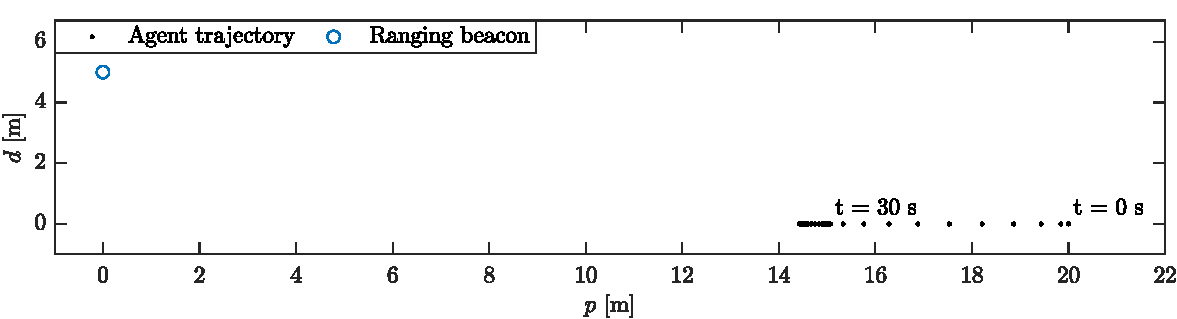
\includegraphics[width=.89\linewidth]{mn1_setup}
%	\caption{\todo{refaire}1D example and agent position trajectory along the x axis}
%	\label{fig:mn1_setup}
%\end{figure}
%We estimate their relative position and velocity based on range observations performed by the following vehicle.
%This kind of estimation problem is typical for collision avoidance in platooning formations.
%As we are interested in the relative motion state, computations are performed in the moving frame of the follower vehicle.
We consider two vehicles moving along a single axis in a platooning configuration.
We estimate relative position and velocity based on range observations from the trailing vehicle.
%This type of estimation problem is typical in collision-avoidance strategies for platoons.
Thus, computations are presented in the trailing vehicle's frame.

Position and velocity dynamics, $p$ and $v$, w.r.t. to the leader
are 
\begin{align}
\label{eq:1D_fx}
\left[\begin{matrix}
    \dot{p}(t)\\\dot{v}(t)
\end{matrix}\right]=\dot{\vec{x}}(t)
&=
\left[\begin{matrix}
v(t)\\
-C_D \abs{v(t)}v(t)+ a(t)
\end{matrix}\right],
\end{align}
%\begin{align}
%\label{eq:1D_fx}
%\left[\begin{smallmatrix}
%    p(t_{k+1})\\v(t_{k+1})
%\end{smallmatrix}\right]=\vec{x}(t_{k+1})
%&=
%\left[\begin{smallmatrix}
%p_k + T_s v_k\\
% v_k - T_s C_D \abs{v_k}v_k + T_s a_k
%\end{smallmatrix}\right]
%+ \vec{q}_k,
%\end{align}
where $C_D$ is the aerodynamic drag, $a$ is the unknown but bounded relative acceleration due to driver inputs.
%and 
The quadratic influence of the velocity on aerodynamic drag requires linearization of \eqref{eq:1D_fx}.
Linearizing around $(\bar{p},\bar{v},\bar{u})$ and using a \zohshort\ yields
\begin{align}
\label{eq:1D_AxBu}
\vec{x}(t_{k+1})
&=
F(t_{k}) \vec{x}(t_{k})
+
Q(t_{k})
a_k
+ \vec{q}_k
+ \epsilon_{\vec{f}}.
+ c_{\vec{f}}.
\end{align}
With ${F(t_{k-1})\!=\!\!\left[\begin{smallmatrix}
1&T_s\\
0& 1 - 2C_D\abs{\bar{v}_k}T_s
\end{smallmatrix}\right]}$, ${Q(t_{k})\!=\!\!\left[\begin{smallmatrix}
  0.5T_s^2 \\ -C_D\abs{\bar{v}_k}T_s^2+T_s \end{smallmatrix}\right]}$,
$\vec{q}_k$ the discretization error,
$\epsilon_{\vec{f}}$ the linearization error and $c_{\vec{f}}$
as in \eqref{eq:czesmf_propa}.

Range sensor observations are susceptible to parametric uncertainty in its inclination angle ${\alpha \in [0, 2] \deg}$:
\begin{align}
r(t_{y,k}) =
p \cos(\alpha)^{-1}
+ w_k,
\label{eq:mn1_h}
\end{align}
with measurement noise ${w_k \in [-0.224, 0.168] \, \mathrm{m}}$.

%\subsection{Initialization}
We assume that initially the vehicles' separation and relative  velocity are confined to
%\begin{align}
${\pre{\set{Z}}_x(t_1) = \set{Z}\left(\begin{smallmatrix}
[0, 1000]\\
0.7\unitInterval
\end{smallmatrix}\right)}.$
%\end{align}
%\subsection{Propagation}
Being the vehicle's acceleration bounded by ${a(t) \in [a] = 0.4\unitInterval \,\mathrm{m}\mathrm{s}^{-2}}$, a \linearinclusion\ for $\vec{x}(t_{k})$ is given by
\begin{align}
\vec{x}(t_{k+1})
\inspacey &
F (t_{k})
\set{Z}_{\vec{x}}(t_{k})
+
\set{Z}_{\vec{q}}(t_{k}),
\label{eq:mn1_f}
\end{align}
with $\set{Z}_{\vec{q}}(t_{k}) = Q(t_k)\set{Z}([a]) $,
and the \apriori\ \cz\ is
\begin{equation}
\pre{\set{Z}}_{\vec{x}}(t_k) =
F
\post{\set{Z}}_{\vec{x}} (t_{k-1})
+
\post{\set{Z}}_{\vec{q}}(t_{k-1}).
\label{eq:mn1_propagation}
\end{equation}
%\subsection{Update}
Since no uncertain observations times are observed in this example, i.e., ${t_k = t_{y,k}}$, we propagate the state enclosure to the observations' time of validity. From \eqref{eq:mn1_h}, we have
\begin{align}
{r}(t_k) \in
H(t_k)
\set{Z}_{\vec{x}}(t_k)
+ \set{Z}([{w}] )
+ \set{Z}([\vec{\epsilon}_{\vec{h}}] )
+ \vec{c}_{\vec{h}}(t_k),
\end{align}
with
${H(t_k)
=
r_{\vec{x}}(\bar{\vec{x}},\bar{\vec{u}})
=
\left[\begin{smallmatrix}
\frac{\bar{p}_k}{\sqrt{d^2 + \bar{p}^2_k}} & 0
\end{smallmatrix}\right]
=
\begin{bmatrix}
H_p & H_v
\end{bmatrix}}$
and\\
${c_{\vec{h}}(t_k) =
 \sqrt{
	d^2 + \bar{p}_k^2
}
-
H(t_k)
\bar{\vec{x}}(t_k)}$.

When computing an enclosure of the linearization error, the generic approach of evaluating the Lagrange remainder \citep{scholte2003nonlinear} by interval arithmetic often leads to overly conservative enclosures due to dependencies. Evaluating $\epsilon_{\vec{h}}$ explicitly can provide tighter enclosures, even more so when exploiting monotonicity \citep{Bolting2018b}. An explicit expression of the linearization error is
${\epsilon_{\vec{h}} =
\norm{\vec{x}}
%\sqrt{d^2 + p^2}
-
H_p
p
- c_{\vec{h}}(t_k)}$.
To check for monotonicity, we can consider the derivative
${{\epsilon_{\vec{h}}}_{p}(p)
=
\frac{p}{\sqrt{d^2 + p^2}}
-
H_p}$.
To compute a tight inclusion of $\epsilon_{\vec{h}}$ over the interval enclosure of the \apriori\ \cz\ $\left[ \hat{Z}_x(t_k) \right]$, we need to evaluate its vertices as well as the possible inflection point given by
${\epsilon_{\vec{h}}}_{p}(\bar{p})
=
0$, i.e.,
 $\bar{p}
=
\sqrt{
	\frac{
H_p d^2
}{
1 - H_p^2
}
}$.
The update is then performed using \eqref{eq:czesmf_update_start},
and conditional reduction with $\bar{n}_g = 6$ and $\bar{n}_c = 2$.\\
Fig.~\ref{fig:mn1_p_and_v} presents \cz\ enclosures and state intervals for position and velocity. It illustrates the behavior of the proposed constrained-zonotope filter on the 1D platooning scenario. The true position and velocity remain enclosed by the estimated sets at all times, confirming the consistency of the approach. As new range observations are incorporated, the enclosures contract due to the strip intersections, while model propagation widens the sets because of bounded acceleration and linearization uncertainties.
%Fig.~\ref{fig:mn1_p_and_v} presents \cz\ enclosures and state intervals. 
% 1D example
%\begin{figure*}
%	\begin{subfigure}{\linewidth}
%		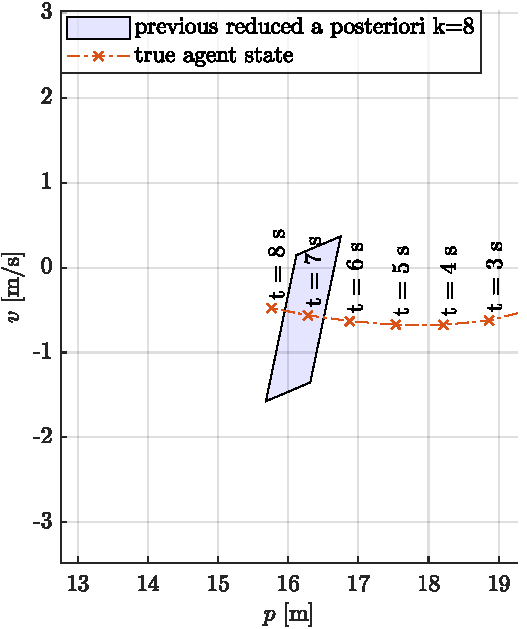
\includegraphics[width=.45\linewidth]{mn1d_bw_closeup_beforepropagation_k=9}\hfill
%		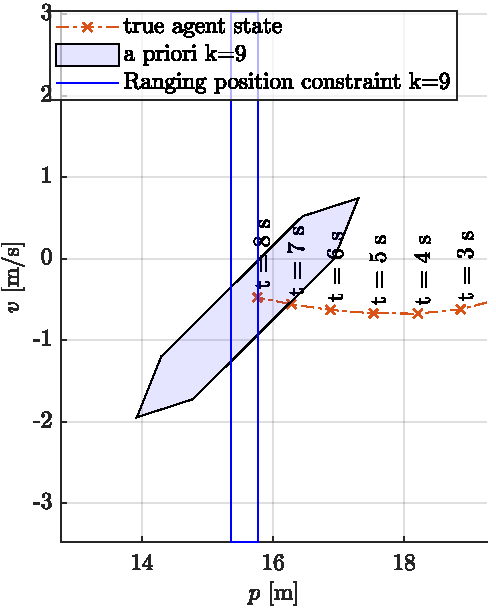
\includegraphics[width=.45\linewidth]{mn1d_bw_closeup_apriori_and_observation_k=9}
%		%	\caption{}
%	\end{subfigure}\par\medskip
%	\begin{subfigure}{\linewidth}
%		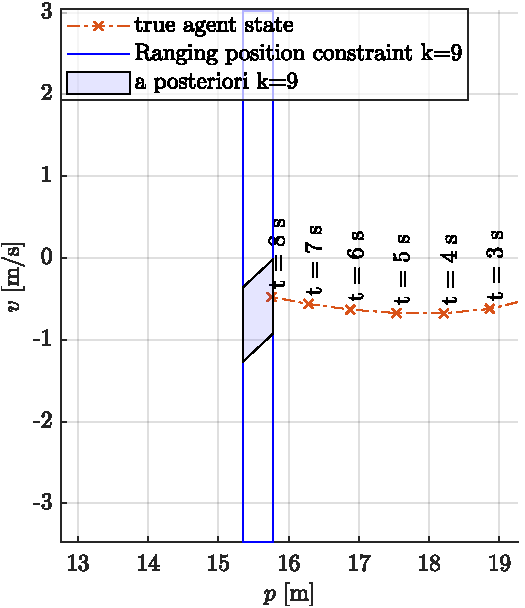
\includegraphics[width=.45\linewidth]{mn1d_bw_closeup_update_k=9}\hfill
%		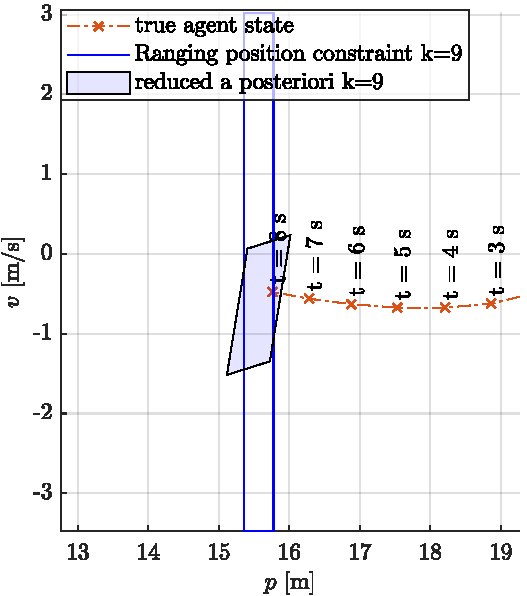
\includegraphics[width=.45\linewidth]{mn1d_bw_closeup_reduction_k=9}
%		%	\caption{}
%	\end{subfigure}\par\medskip
%	\caption{Snapshot of the steps of the 1D example}
%	\label{fig:mn1_steps}
%\end{figure*}

%\begin{figure*}
%	\centering
%	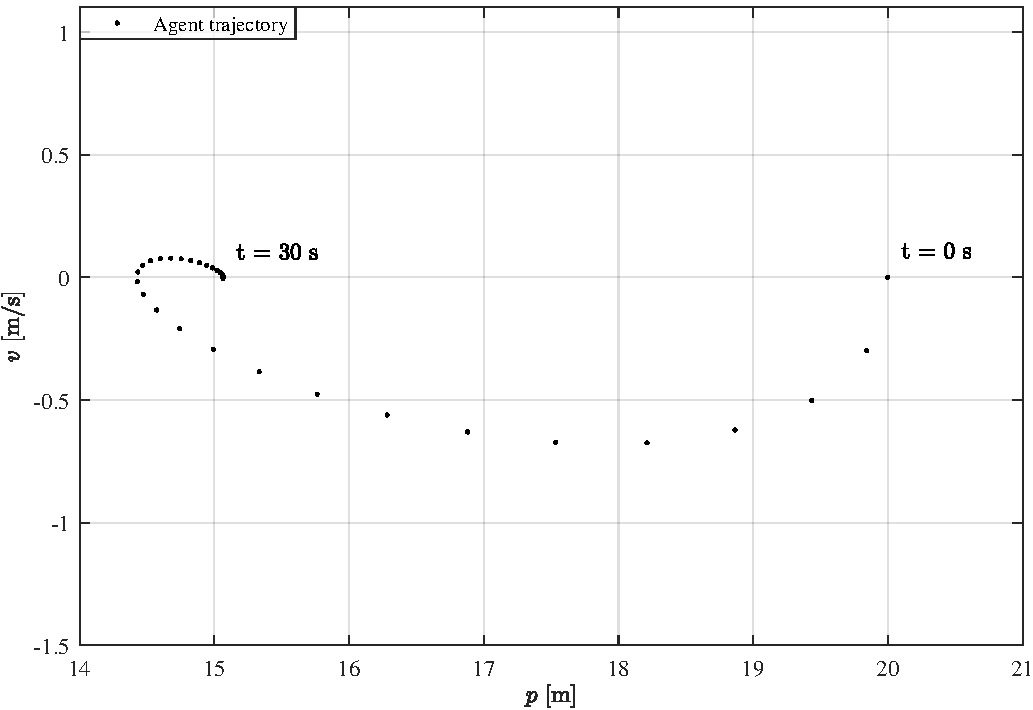
\includegraphics[width=.45\linewidth]{mn1_trajectory_initial}
%	\caption{1D example: state trajectory, agent position and velocity}
%	\label{fig:mn1_trajectory_initial}
%\end{figure*}
\begin{figure}[b!]
	\centering
%	\caption{1D example: state trajectory and enclosures.}	\label{fig:mn1_trajectory}
% \begin{subfigure}{\linewidth}
	% \centering
    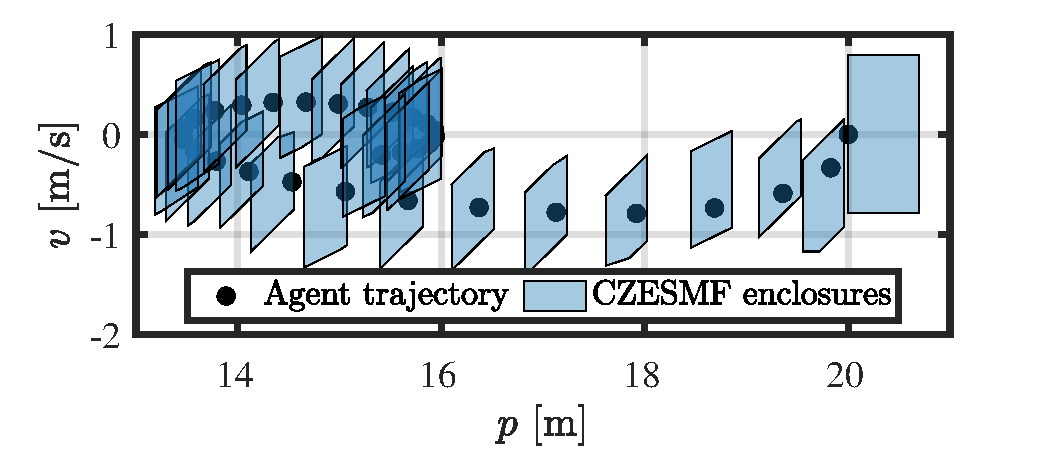
\includegraphics[width=.7\linewidth]{mn1_trajectory}
    
	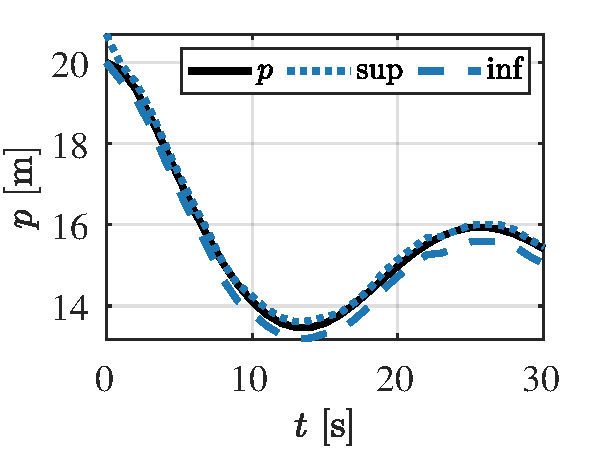
\includegraphics[width=.4\linewidth]{mn1_p}
% 	\caption{}
% 	\label{fig:mn1_p}
% \end{subfigure}
% \begin{subfigure}{\linewidth}
% 	\centering
	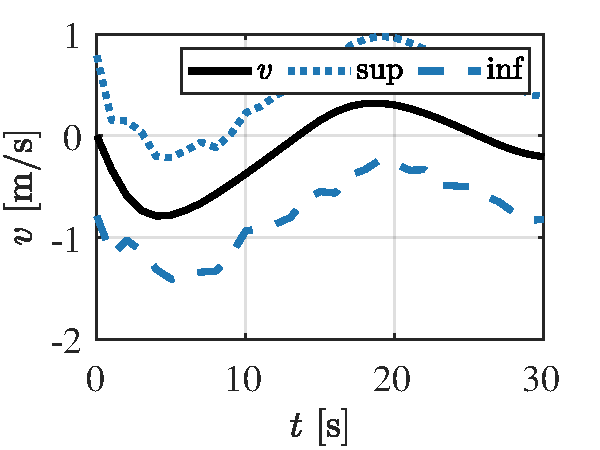
\includegraphics[width=.4\linewidth]{mn1_v}
	
	% \caption{}
% 	\label{fig:mn1_v}
% \end{subfigure}
	\caption{\cz\ enclosures and position and velocity intervals.}
	\label{fig:mn1_p_and_v}
\end{figure}


\subsection{2D localization --- Vehicle tracking in urban traffic roads}\label{sec:example_2D}
\vspace{-0.2cm}
The second example considers a vehicle moving in a two-
dimensional environment with static ranging beacons and uncer-
tain observation times. The ranging capabilities may be provided
by urban infrastructure, such as smart lamp posts or smart traffic lights,
or by low-cost \uwbshort\ devices in
indoor environments.
%This example consists of a vehicle moving in an  environment with static ranging beacons with uncertain observation times. 
%The ranging capabilities can be served via the urban infrastructure, e.g., through smart lamp posts or smart traffic lights.
%The same example can be reproduced in a smaller scale using low-cost \uwb. 

%This represents real case scenarios such as automatic lawnmowers or lift trucks in a modern warehouse.
We assume the vehicle's position
${\vec{x} = \left[x_1 \; x_2\right]^T}$
is governed by
\begin{equation}
  \vec{x}(t_{k+1}) = \vec{x}(t_{k}) + \vec{q}(t_{k}),
  \label{eq:mn_f}
\end{equation}
where
%\begin{equation}
${\norm{\vec{q}(t_k)} \leq \bar{v} (t_{k} - t_{k-1})}$,
%  \label{eq:mn_qball}
%\end{equation}
$\bar{v}$ the maximum velocity. 

\begin{remark}
  The bound $\bar{v}$ may correspond, for instance, to the terminal velocity of a system with quadratic drag under maximum input acceleration. This conservative model can be adopted when more detailed knowledge of the inner dynamics is unavailable.
  %$\bar{v}$ may correspond to the terminal velocity of a system with quadratic drag under maximum input acceleration.
 % This conservative model can be used when better knowledge of inner dynamics is unavailable.
\end{remark}

The vehicle receives regularly ranging observations from beacons situated at uncertain positions
\begin{align}
  \vec{p}_{bi} \in
  \overline{\vec{p}_{bi}}+
 \left[\begin{smallmatrix}
    0.1& 0.1
  \end{smallmatrix}\right]^T
  \unitInterval =\overline{\vec{p}_{bi}} +
  \epsilon_b
\end{align}
with $\overline{\vec{p}_{b1}}=\left[\begin{smallmatrix}
    10& 10
\end{smallmatrix}\right]^T$,
$\overline{\vec{p}_{b2}}=\left[\begin{smallmatrix}
    -10& -10
\end{smallmatrix}\right]^T$ and
$\overline{\vec{p}_{b3}}=\left[\begin{smallmatrix}
    10& -10
\end{smallmatrix}\right]^T$.

We simulate the vehicle's movement for a total of $\qty{20}{\second}$.
During this interval, we assume the vehicle receives ranging observations from the beacons resulting in $k=63$ observations.
The observed ranging and timestamps received from each beacon $i_k$ are described as
\begin{align}
  \left[\begin{smallmatrix}
    r_k \\ t_{y,k}
  \end{smallmatrix}\right]
  &=
    \left[\begin{smallmatrix}
      ||\vec{x}(t) - \vec{p}_{b i_k} || \\
      t + w_t(t)
    \end{smallmatrix}\right].
    \label{eq:mn_h}
\end{align}
The nominal observation frequency is $\qty{1}{\Hz}$.
However, synchronization issues between the sensors and walltime cause jitter, with ${\rad{[w_t]}=0.01\unit{\s}}$.
%These observations arrive in a nominal frequency of $\qty{1}{\Hz}$.
%However, synchronization issues between the sensors and walltime causes jittering, ${\rad{[w_t]}=0.01\unit{\s}}$.

Fig.~\ref{fig:mn_trajectory_initial} illustrates the intervals corresponding to the beacons' positions, the trajectory of the vehicle, which presents a sharp bend, and an estimation of the enclosure of the state $\vec{x}$ at time ${t=\qty{0}{\second}}$, whose estimation will be detailed in the following.
\begin{figure}[h]
  \centering
  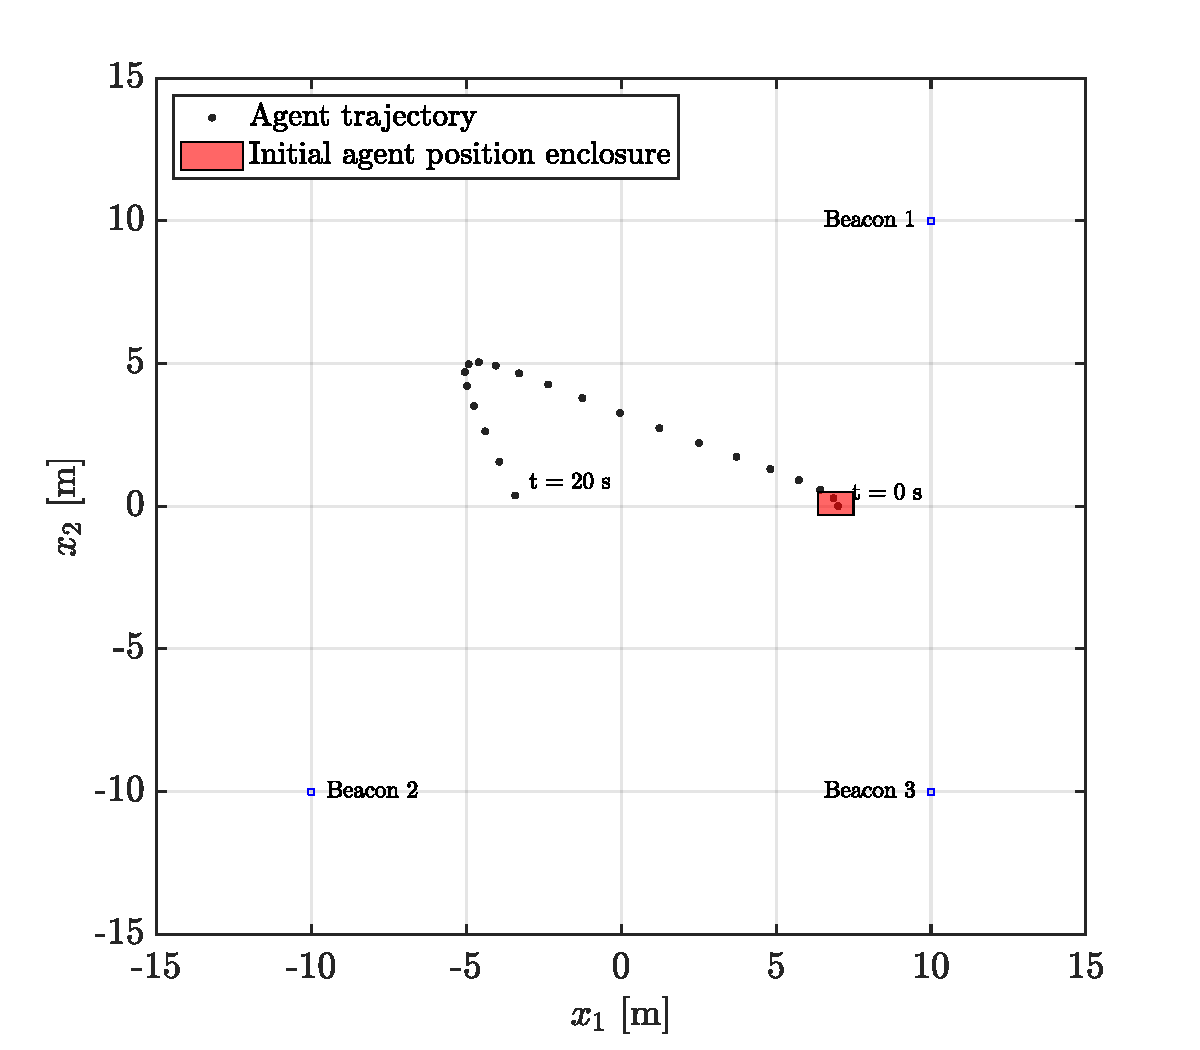
\includegraphics[height=.55\linewidth,clip,trim=0 10 0 30]{../img/trajectory_initial_form3.pdf}
  \caption{2D localization problem with full vehicle trajectory.}% and initial position enclosure obtained by \vsivia{}.}
  \label{fig:mn_trajectory_initial}
\end{figure}

\subsection{Initialization}\label{sec:initialization_example}
\vspace{-0.2cm}
%Since we know that the agent is initially inside the field, we can compute a \cz\ covering the field and use it as an initial \cz\ for our algorithm.
%While the field-covering \cz\ is valid, it is an extremely conservative initial enclosure, leading to extremely conservative filter solutions due to wrapping effect.
%As a palliative measure,
As initial \cz, we use an interval enclosure of a paving calculated using the \vsivia\ (see Fig.~\ref{fig:mn_visivia}).

%\begin{remark}
%This one-time 2D \vsivia\ estimation takes about $\qty{0.5}{\s}$ and processes $369$ boxes with ${\epsilon = \qty{0.05}{\m}}$.
%We can observe that while for a single step it is acceptable, this computation time is too slow to perform in an real-time embedded system.
%Observe also that for problems in higher state dimensions, it might be preferable to couple \vsivia{} with constraint propagation to compute a sufficiently tight initial state enclosure in an acceptable time.
%\end{remark}

\begin{figure}[tb]
  \centering
  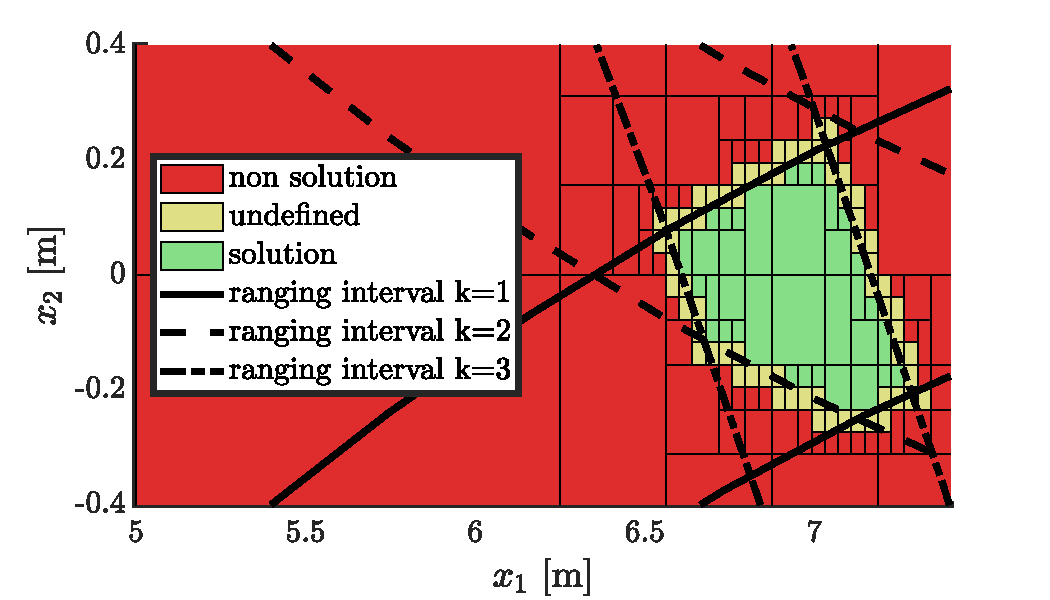
\includegraphics[width=.7\linewidth,clip,trim=0 0 0 15]{../img/3beacons_form3_obstimrad0.01_czesmf_results_vsivia.pdf}
  \caption{Subpaving of initial position using range observations.}
  \label{fig:mn_visivia}
\end{figure}

%\subsection{Propagation}
Since dynamics are linear, state propagation is 
\begin{equation}
  \pre{\set{Z}}_{\vec{x}} (t_k) =
  \set{Z}(t_{k-1})
  + \set{Z}_s(t_{k-1}),
  \label{eq:mn_propagation}
\end{equation}
where $\set{Z}_s(t_k)$ is a \cz\ over-approximation of the ball of radius $\bar{v}(t_{k} - t_{k-1})$, e.g., a box.

% \begin{figure}
%   \centering
%   \includegraphics[width=.99\linewidth]{mn_closeup_apriori_k=9}
%   \caption{2D localization problem: Preceding reduced \aposteriori\ \cz, \apriori\ \cz. Best viewed in color.}
%   \label{fig:mn_propagation}
% \end{figure}
%\subsection{Update}
We perform sequential updates in the nominal frame of the ranging beacon $i_k$, which corresponds
to a \apriori\ \cz\ in the beacon frame 
%\begin{align}
  $\pre{\set{Z}}^b_{x} (t_k) = \pre{\set{Z}}_{\vec{x}} (t_k) - \vec{p}_{b i_k}$.
%\end{align}
%
Then, each ranging observation is rewritten
${r(t_{k}) = ||\vec{x}(t_{k}) - \epsilon_b|| + w_{r,k}}$.
To simplify, we absorb the small beacon uncertainty into the observation error $w_{r,k}$
%by using the inequality
%$\norm{\vec{x}} - \norm{\epsilon_b}  \geq \norm{\vec{x} - \epsilon_b} \leq \norm{\vec{x}} + \norm{\epsilon_b}$,
yielding
\begin{align}
  r(t_{k}) = \norm{\vec{x}(t_{k})} + w'_{r,k},
  \label{eq:mn_h2}
\end{align}
with ${w'_{r,k} \in [w'_r] = [w_{r}] + \rad{[\epsilon_b]} \unitInterval}$.

From~\eqref{eq:mn_h2}, we construct the \linearinclusion\
\begin{align}
  {r}(t_{k}) \in
                         H_{\vec{x}}(t_k)
                         \set{Z} (t_{k})
                         + \set{Z}([w'_r] )
                         + \set{Z}([\epsilon_h])
                         + c_h(t_k)
\end{align}
with
  ${H_{\vec{x}}(t_k) = \dir(\bar{\vec{x}}^T(t_k))}$
and
${c_h(t_k) = \norm{\vec{x}_k} - H_{\vec{x}}({t_k}) \bar{\vec{x}}(t_k)}$.

%\subsubsection{Observation interval inflation}\label{sec:observation_interval_inflation}
To adjust for timing jitter, we compute the necessary state increment $[\Delta \vec{x}(t_k)]$ from the velocity norm bound $\bar{v}$
\begin{align}
  [\Delta \vec{x}] = \bar{v} \, \rad{[w_t]}
  \1_2\unitInterval.
\end{align}
Then, we inflate the observation inclusion
\begin{align}
  {r}(t_{y,k}) \in\,&
                           H_{\vec{x}}(t_k)
                           \set{Z}^b_{\vec{x}} (t_k)
                           + \set{Z}([w'_r] )
                           + \set{Z}([\epsilon_h])\nonumber\\
                    &       + c_h(t_k)
                           + H_{\vec{x}}(t_k) \set{Z}([\Delta \vec{x}]).
\end{align}
After computing $\post{\set{Z}^b}_{\vec{x}}(t_k)$ using~\eqref{eq:czesmf_update_start}, the \cz\ is translated back to the navigation frame:
\begin{align}
  \post{\set{Z}}_{\vec{x}} (t_k) = \post{{\set{Z}}^b}_{\vec{x}} (t_k) + \vec{p}_{b i_k}.
\end{align}

% \begin{figure}
%   \centering
%   \includegraphics[width=.99\linewidth]{mn_closeup_reduction_k=9}
%   \caption{2D localization problem: Update with original and reduced \aposteriori\ \cz. Best viewed in color.}
%   \label{fig:mn_update}
% \end{figure}
% 2D example
%\begin{figure*}[h]
%  \begin{subfigure}{\linewidth}
%    \includegraphics[width=.45\linewidth]{mn_bw_closeup_beforepropagation_k=9}\hfill
%    \includegraphics[width=.45\linewidth]{mn_bw_closeup_apriori_and_observation_k=9}
%    %	\caption{}
%  \end{subfigure}\par\medskip
%  \begin{subfigure}{\linewidth}
%    \includegraphics[width=.45\linewidth]{mn_bw_closeup_update_k=9}\hfill
%    \includegraphics[width=.45\linewidth]{mn_bw_closeup_reduction_k=9}
%    %	\caption{}
%  \end{subfigure}\par\medskip
%  \caption{Filter steps of the 2D example, observation timing noise 0.01 s}
%  \label{fig:mn_0.01}
%\end{figure*}

%\begin{figure*}[h]
%  \begin{subfigure}{\linewidth}
%    \includegraphics[width=.45\linewidth]{mn_bw_closeup_beforepropagationdThigh_k=9}\hfill
%    \includegraphics[width=.45\linewidth]{mn_bw_closeup_apriori_and_observationdThigh_k=9}
%    %	\caption{}
%  \end{subfigure}\par\medskip
%  \begin{subfigure}{\linewidth}
%    \includegraphics[width=.45\linewidth]{mn_bw_closeup_updatedThigh_k=9}\hfill
%    \includegraphics[width=.45\linewidth]{mn_bw_closeup_reductiondThigh_k=9}
%    %	\caption{}
%  \end{subfigure}\par\medskip
%  \caption{Filter steps of the 2D example, observation timing noise 0.1 s}
%  \label{fig:mn_0.1}
%\end{figure*}

%Fig.~\ref{fig:mn_0.01} shows the obtained \aposteriori\ \cz\ at $t_9$, as well as the reduced \aposteriori\ \cz.
%Fig.~\ref{fig:mn_0.01} and shows the obtained results with increased timing noise. Note the larger \aposteriori\ \cz\ due to increased observation interval inflation.

% illustrating the trade off between complexity and conservatism.
%
In Fig.~\ref{fig:czs_prior_posterior}, we can see an example of an usual \czesmf\ recursion.
We show the iteration for $t_{10}$.
Observe that the \aposteriori\ \cz\ for time $t_9$, i.e., $\post{\set{Z}}(t_{9})$, is propagated to generate the \apriori\ $\pre{\set{Z}}(t_{10})$.
Once the observation is received and corrected for the jittering, it is intersected with $\pre{\set{Z}}(t_{10})$ resulting in the complex $\set{Z}'(t_{10})$.
Finally, the reduction is triggered, resulting in the less complex but more conservative $\post{\set{Z}}(t_{10})$.
\begin{figure}[hb]

  \centering
  \resizebox*{!}{3.5cm}{
  \footnotesize
  \def\svgwidth{1.2\linewidth}
  \import{../img/}{czesmf_prior_and_posterior_10_latex.pdf_tex}}%
  \resizebox*{!}{3.5cm}{
  \footnotesize
  \def\svgwidth{1.2\linewidth}
  \import{../img/}{czesmf_prior_and_posterior_10_2_latex.pdf_tex}}
  %	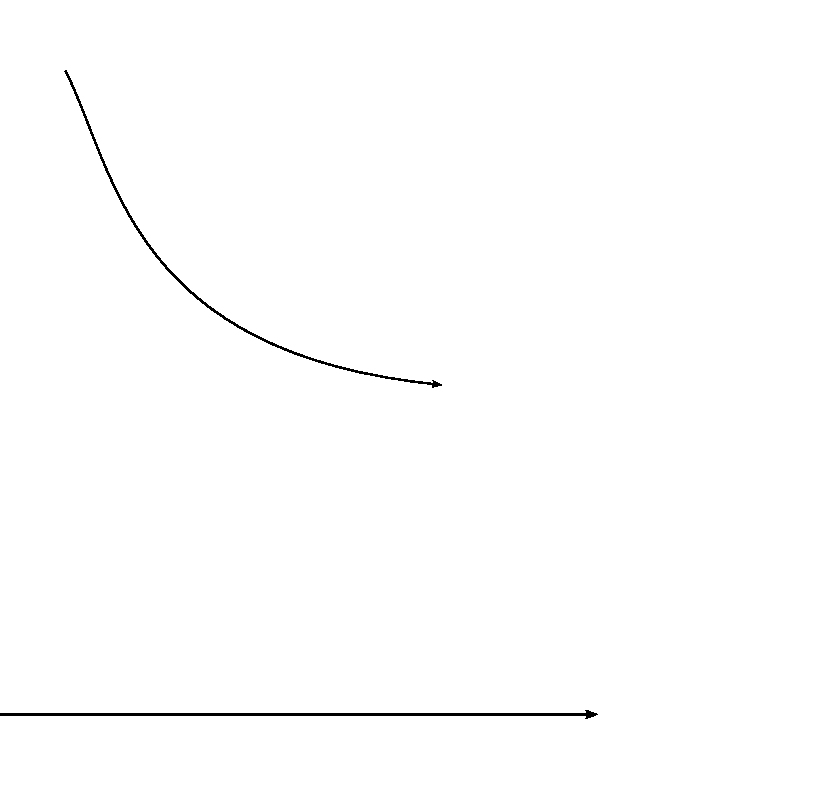
\includegraphics[width=.99\linewidth]{timing.pdf}
  \vspace{-.25cm}
  \caption{Sets in a \czesmf\ recursion. Timing noise $\qty{0.01}{\second}$.%, $k=10$.
  }
  \label{fig:czs_prior_posterior}
\end{figure}

% \glsstepentry{\vsvia}
% \glsstepentry{\vsivia}
\subsubsection{Results}
We compare the four algorithms (\czesmf, \vsiviashort, \iesmf\ and \ekf) w.r.t. the volume of the estimated sets and the execution times in different scenarios with increasing observation timing errors, $\rad{[w_t]}\in \{0.01,0.05,0.1,0.5\}\unit{\s}$.
%Figures~\ref{fig:mn_trajectory} and \ref{fig:mn_trajectory_dtHigh} present the \czs\ for observation timing errors $\qty{0.01}{\second}$ and $\qty{0.1}{\second}$ respectively.
%Observe that due to bigger timing errors, the ranging observations do not necessarily arrive at the right order and, as a remedy, the algorithm inflates the observation interval (\S\ref{sec:observation_interval_inflation}).
%An increased timing error leads to a bigger inflation and consequently bigger enclosures.

%\begin{figure}[h!]
%  \centering
%  
\includegraphics[width=\linewidth]{figures/trajectory_obstimrad0.01_form3.pdf}
%  \caption{Estimated \czs. Timing noise $\qty{0.01}{\second}$.}
%  \label{fig:mn_trajectory}
%\end{figure}

%\begin{figure}[h!]
%  \centering
%  
\includegraphics[width=\linewidth]{figures/trajectory_obstimrad0.1_form3.pdf}
%  \caption{Estimated \czs. Timing noise $\qty{0.1}{\second}$.}
%  \label{fig:mn_trajectory_dtHigh}
%\end{figure}
%
%
For the \czesmf\ implementation, we use the parameters ${\bar{n}_g = 15}$, ${\bar{n}_c = 1}$ and ${\overline{\Delta t}=\qty{0.01}{\second}}$.
For the \vsiviashort\ implementation, we 
propagate the subpavings interval hull between two updates. We use interval hulls  since subpavings are not closed under the propagation, i.e., the result is not necessary a non-overlapping interval bundle. We choose ${\epsilon=0.05}$ as the length of the minimal boxes.
For the \iesmf, we used ${N=10}$ iterated updates with the \emph{trace} metric~\citep{Bolting2018b}.
To compare with \ekf, we use $3\sigma$ confidence ellipsoids.

In Fig.~\ref{fig:mn_compare_volumes_k_3}, we show the estimated sets produced by the different algorithms for a given observation ${k=3}$.
As the subpaving generated by \sivia\ may contain hundreds of boxes, we display its convex hull for readability.

%In Fig.~\ref{fig:mn_compare_volumes_k_3}, we see the estimated sets by the different algorithms for a given observation ${k=3}$.
%As we can see, the resulting subpavings of the \sivia\ is formed by hundreds of boxes, to simplify visualization we use its convex hull.

\begin{figure}[htb]
  \centering
  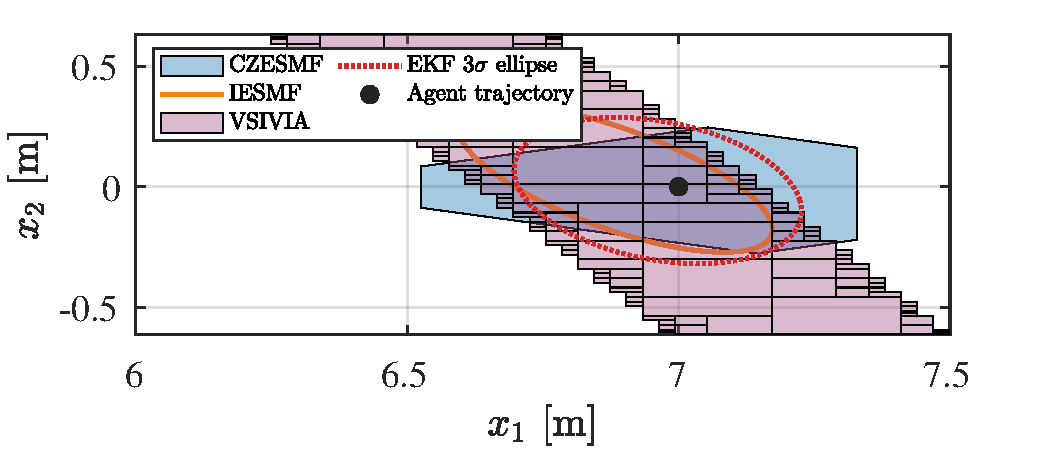
\includegraphics[width=.8\linewidth,clip,trim=0 0 0 15]{../img/comparison_volumes_czesmf_ekf_obstimrad0.01_k_3.pdf}
  \vspace{-.25cm}
  \caption{Estimated sets for ${k=3}$. Timing noise $\qty{0.01}{\second}$.}
  \label{fig:mn_compare_volumes_k_3}
\end{figure}

%\begin{remark} As one can notice, the subpaving from \vsivia\ is bigger than the ones estimated by \iesmf\ and \czesmf.
%The causes of the conservatism are twofold.

%A first cause is the over-approximation of the propagated state subpaving by a box before performing the update.
%This approximation provokes a wrapping effect and reduces the advantages of \vsivia\ when approximating non-convex sets.
%Further research should be directed towards the conditional propagation of the subpavings.

%The second cause is intrinsic to the hypothesis of the experiment.
%As we suppose the ranging observations of the beacons arrive in different times, the \vsivia\ can only use one observation at a time, resulting in an annulus sector (as seen in \ref{fig:mn_compare_volumes_k_3}).
%Since the target is moving, from one observation to another, it is possible it's position is not enclosed anymore by the \aposteriori\ set calculated using the previous observation, and then, the intersection of this set with the next observation would result in an empty set, thus the need to propagate the set.
%\end{remark}
\begin{figure}[tb]
  \centering
  \begin{subfigure}{.4\linewidth}
  \centering
  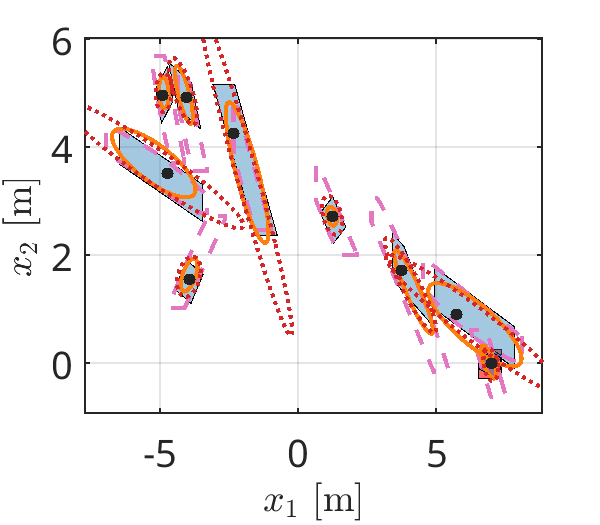
\includegraphics[width=\linewidth,clip,trim=0 4 0 14]{../img/comparison_czesmf_ekf_obstimrad0.01_form3.pdf}
  \caption{Timing noise $\qty{0.01}{\second}$}
  \label{fig:mn_trajectory_ekf_vs_cz__001}
  \end{subfigure}
  \begin{subfigure}{.4\linewidth}
  \centering
 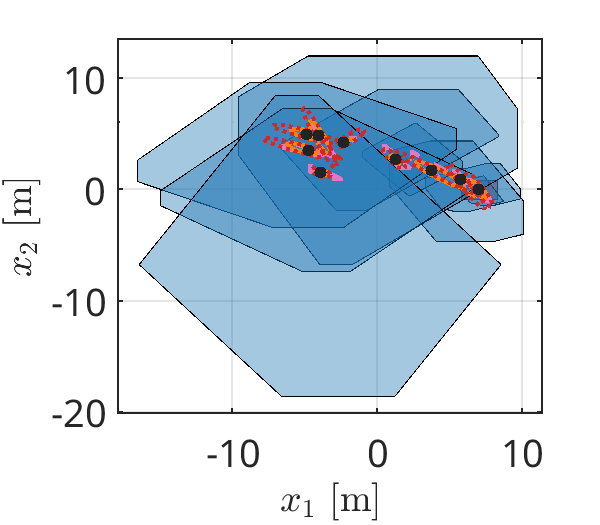
\includegraphics[width=\linewidth,clip,trim=0 4 0 14]{../img/comparison_czesmf_ekf_obstimrad0.5_form3.pdf}
  \caption{Timing noise $\qty{0.5}{\second}$}
  \label{fig:mn_trajectory_ekf_vs_cz_05}
  \end{subfigure}  
\begin{subfigure}{\linewidth}
  \centering
  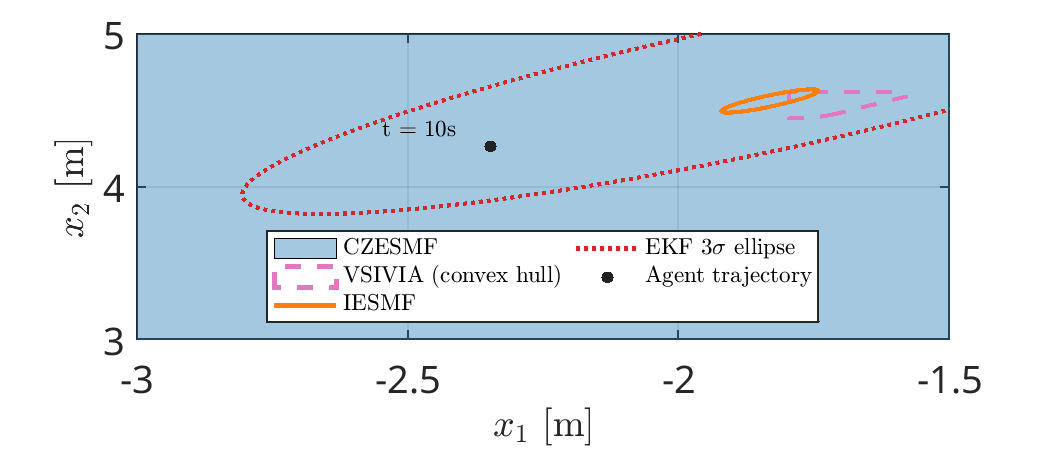
\includegraphics[width=.7\linewidth,clip,trim=0 5 0 11]{../img/comparison_czesmf_ekf_obstimrad0.5_form3_detail_1.pdf}
  \caption{Detail of (b)}
  \label{fig:mn_trajectory_ekf_vs_cz_05_detail}
\end{subfigure}
  
  % \caption{Estimated sets (some omitted for readability). Timing noises $\qty{0.01}{\second}$ (a) and $\qty{0.5}{\second}$ (b). (c) details (b) for $t_{31}=10\unit{\s}$.
  \vspace{-0.2cm}
  \caption{Estimated sets selected for readability.
}\label{fig:mn_trajectory_ekf_vs_cz_001_05}
\end{figure}

Fig.~\ref{fig:mn_trajectory_ekf_vs_cz_001_05} compares the estimated sets for different timing noises. As expected, the volume for \czesmf's sets increases w.r.t the observation timing noise due to the inflation procedure.
However, Fig.~\ref{fig:mn_trajectory_ekf_vs_cz_05_detail} shows that although the smaller sets of other algorithms, they do not necessarily enclose the true state when observation time errors are ignored.
For small timing errors, the estimated sets may coincidentally contain the true state, but as the timing uncertainty grows, discrepancies become apparent.
This highlights the effectiveness of the proposed strategy in limiting conservatism while guaranteeing inclusion of the true state.
%One of the main results of this work can be observed on Figure~\ref{fig:mn_trajectory_ekf_vs_cz_001_05}. It
%compares the estimated sets for different timing noises.
%Observe the increase of the volume of the \czesmf's sets when there is an increase in the observation timing noise.
%However, if we observe Fig.~\ref{fig:mn_trajectory_ekf_vs_cz_05_detail}, which is a detail of Fig.~\ref{fig:mn_trajectory_ekf_vs_cz_05} for $t_{31}$, we see that while the other algorithms can produce smaller sets, they not necessarily enclose the true position, since observation time errors are ignored.
%or smaller observation errors, coincidentally the sets contain the true trajectory, but as observation errors grow larger, the discrepancy becomes apparent. This emphasizes the effectiveness of the proposed strategy for reducing the conservatism as much as possible while guaranteeing to enclose the real state. 

Fig.~\ref{fig:mn_trajectory_ekf_vs_cz_volume_001_01} shows the evolution of the volumes of the estimated sets for ${\rad{[w_t]}\in\{0.01,0.1\}\unit{\s}}$.
The oscillatory behavior results from alternating propagation and update steps. Every three observations, when information from all beacons is available, the algorithms can perform trilateration and the volumes contract. For small timing errors (${\rad{[w_{t}]}\sim 0.1T_{s}}$), the \czesmf\ generates sets with sizes comparable to those of the other methods.

%Observe in Fig.~\ref{fig:mn_trajectory_ekf_vs_cz_volume_001_01} the evolution of the volume of estimated sets for ${\rad{[w_t]}\in\{0.01,0.1\}\unit{\s}}$.
%The oscillatory behavior is result of iterated propagations and updates. At each $3$ observations, when information of all beacons is used, the algorithms can perform the trilateration and volumes contract.
%As we can see, for small errors ($\rad{[w_{t}]}\sim 0.1T_{s}$), \czesmf\ generated \czs\ with sizes comparable to the others.

Table~\ref{tab:comparison_time} reports the mean execution times of the different methods for four levels of observation time error. Computations were performed on an Intel i7-10610U CPU under MATLAB. Even with a non-optimized implementation, \czesmf\ runs in a fraction of the time required by \vsivia, indicating its potential for embedded applications. Compared with \iesmf, the execution time is larger due to \cz\ operations and occasional reductions, but remains compatible with real-time constraints.% for the considered examples.

%In Table~\ref{tab:comparison_time}, we compare the mean execution time of the iterations of the methods for 4 different observation errors.
%The computations were executed on an Intel i7-10610U CPU.
%As we can see, even with a non optimized implementation, \czesmf\ is still executed in a fraction of the \vsivia's time, indicating potential for embedded applications.
%Comparing with the \iesmf, execution time is bigger due to \czs' operations and occasional reductions.

\section{Conclusions}\label{sec:conclusion}
\vspace{-0.2cm}
This paper proposed a \cz-based \smf\ for nonlinear systems, specifically designed to address uncertainties in observation times. 
\czesmf\ accounts for asynchronous and jittered timestamps by inflating observation intervals, and can incorporate multiple propagation models and parametric uncertainty in the observation equation. Its performance has been evaluated in a 2D vehicle localization problem with increasing observation time errors, and compared with three alternative methods: one based on SIVIA, a fast ellipsoidal set estimator (IESMF), and the widely used \ekf.
The results show that \czesmf\ maintains guaranteed state enclosures even for significant timing errors while achieving reasonable compromise between tightness and computation time, differently from the known methods shown. For small timing uncertainties, the volumes of the sets generated by \czesmf\ are comparable to those of the other methods.

While the implementation used in this study is interpreted and not optimized, execution times indicate potential applicability in embedded systems using low-cost off-the-shelf hardware. Future work will focus on experimental validation on robotic platforms equipped with ranging technologies, and integration of richer motion and observation models.% including more complex vehicle dynamics and multi-sensor fusion schemes.
%This paper proposes a \smf\ for nonlinear systems based on \czs, designed to address observation timing errors.
%Performance is compared in terms of both volume and execution time against existing methods through a 2D vehicle localization problem with increasing observation errors. 
%%: a nonlinear offline set estimator based on SIVIA, a fast ellipsoidal set estimator, and the widely-used Extended Kalman Filter (EKF).
%While the implementation presented is interpreted, results indicate potential application in embedded systems using low-cost off-the-shelf hardware, subject of current work, besides integrating multiple propagation and observation models.

\begin{figure}[tb]
\centering
  \begin{subfigure}{\linewidth}
  \centering
  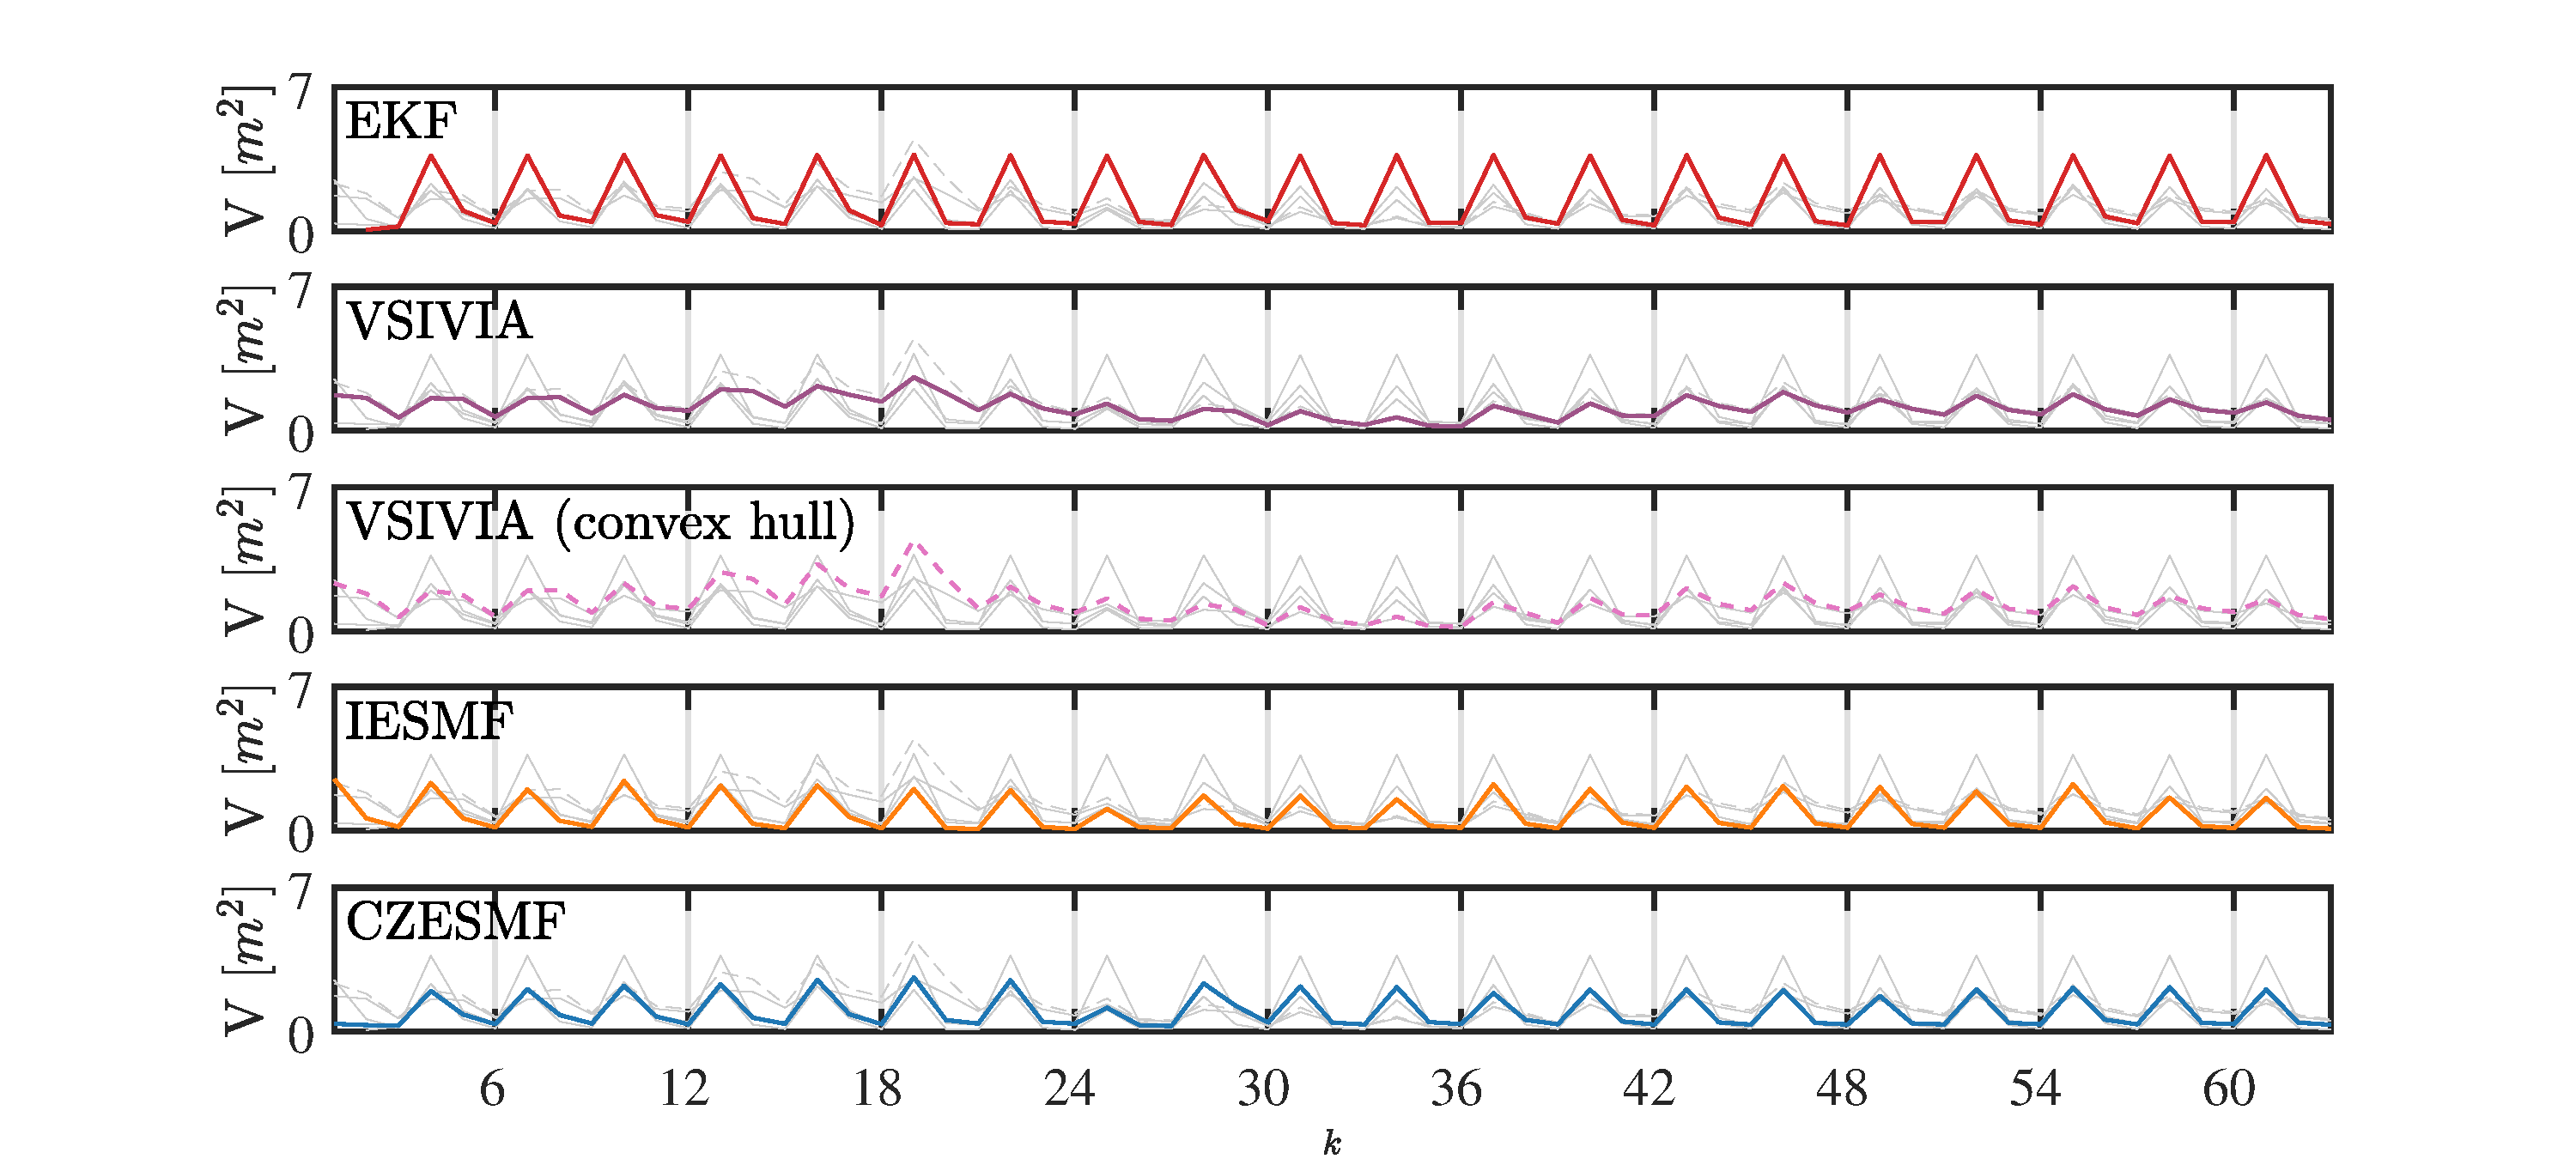
\includegraphics[width=.8\linewidth,clip,trim=0 0 0 35]{../img/comparison_volumes_czesmf_ekf_obstimrad0.01_form3_no_chartjunk.pdf}
  \caption{Timing noise $\qty{0.01}{\s}$. }\label{fig:mn_trajectory_ekf_vs_cz_volume_001}
  \end{subfigure}
  
  \begin{subfigure}{\linewidth}
  \centering
  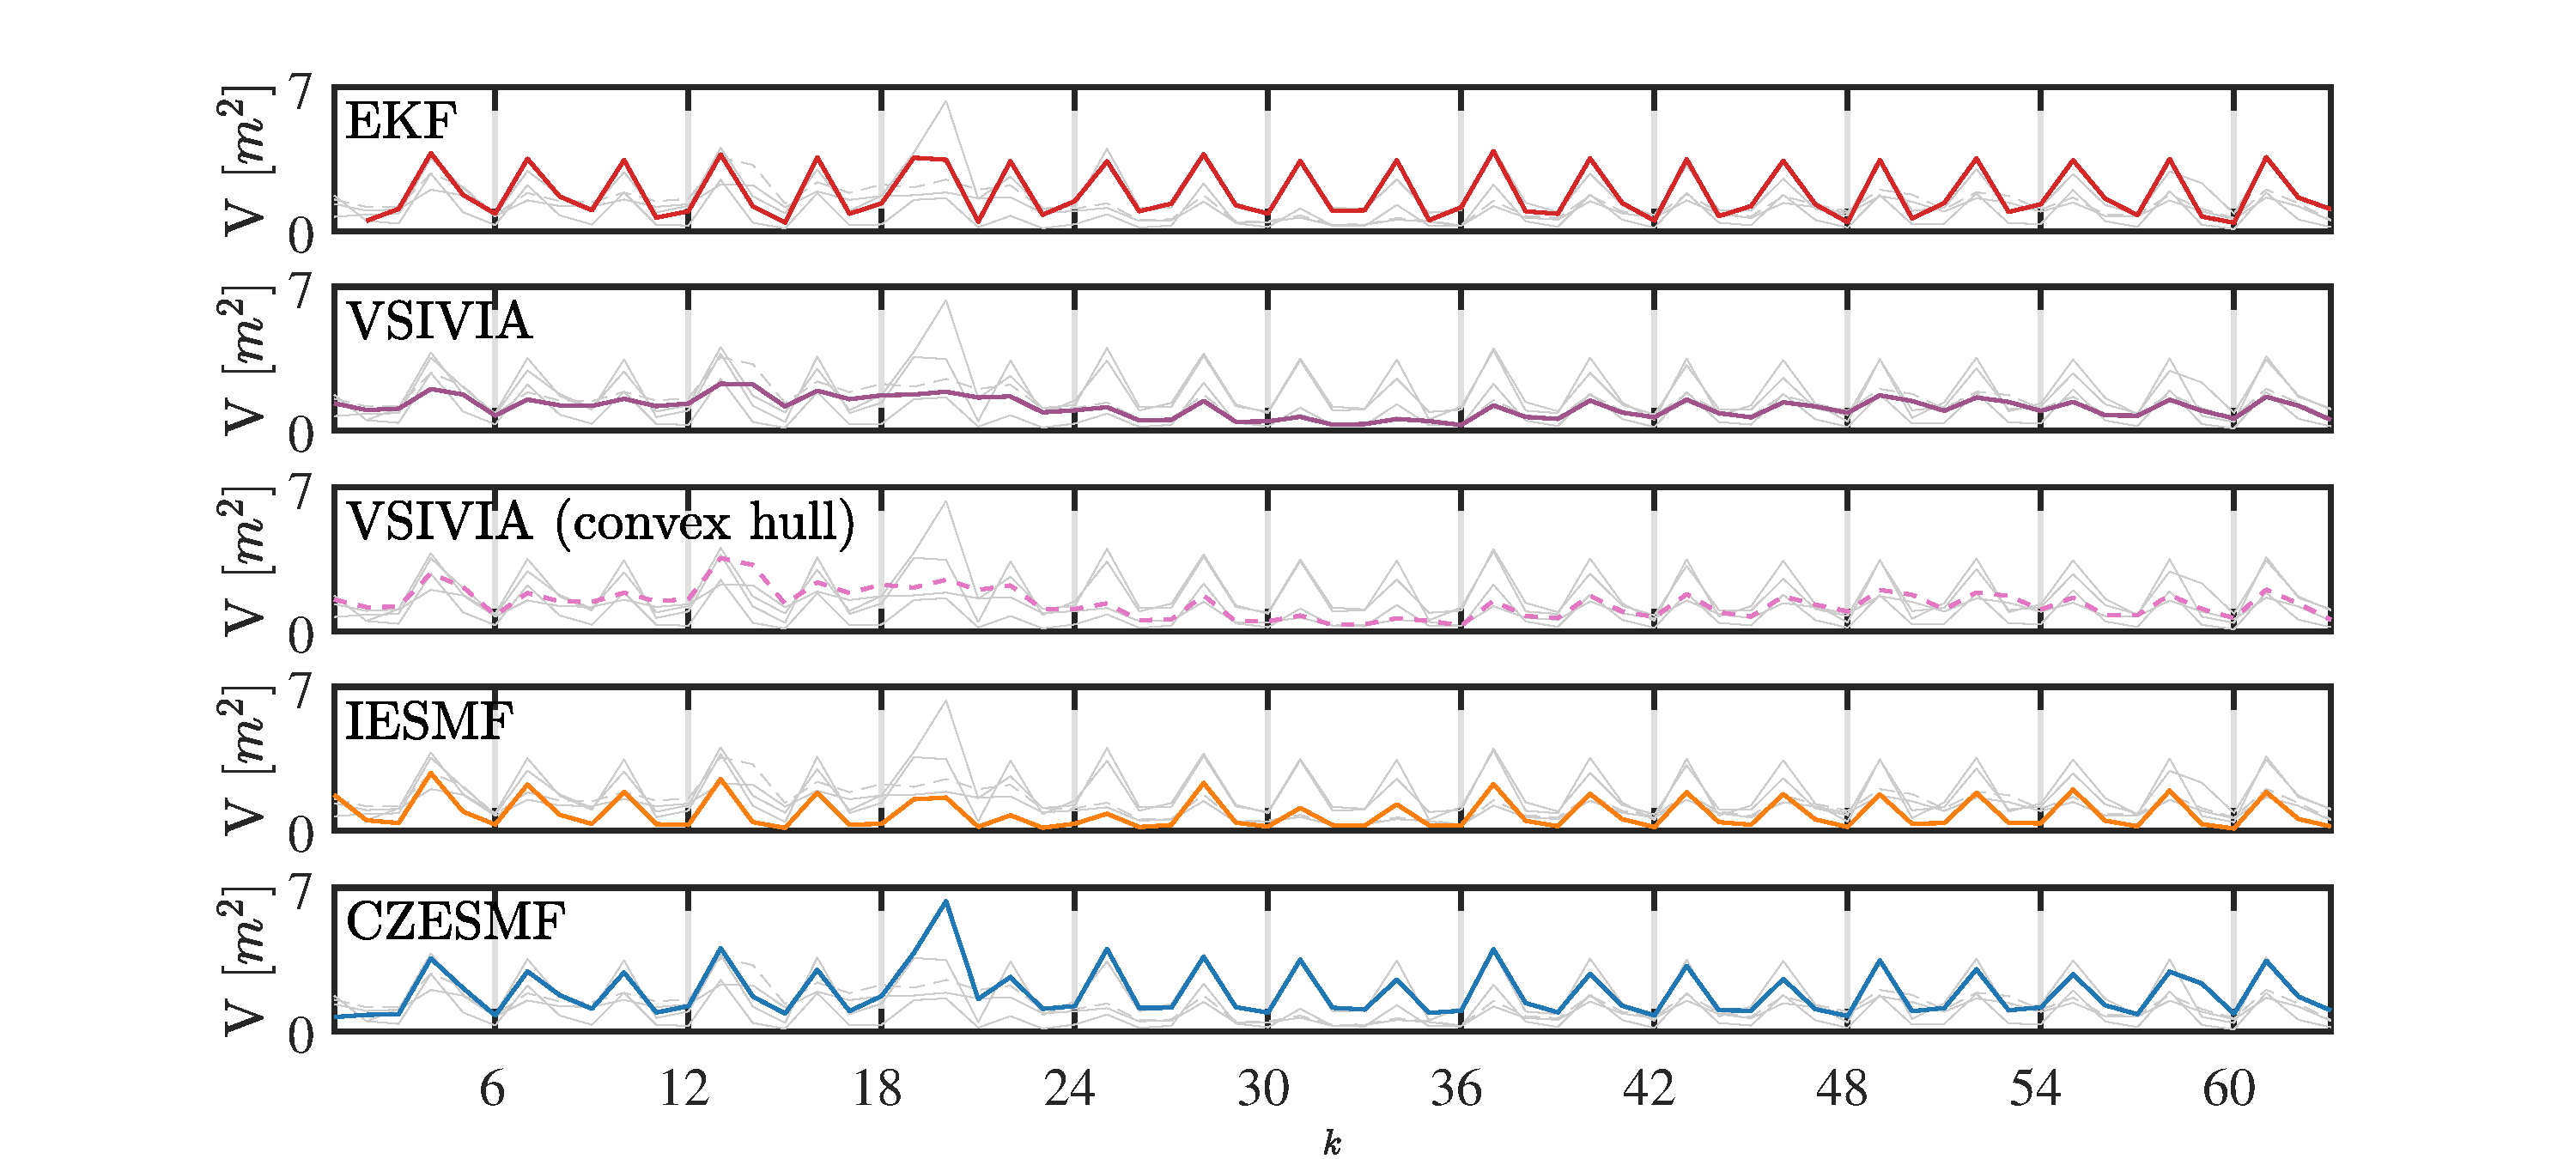
\includegraphics[width=.8\linewidth,clip,trim=0 0 0 35]{../img/comparison_volumes_czesmf_ekf_obstimrad0.1_form3_no_chartjunk.pdf}
  \caption{Timing noise $\qty{0.1}{\s}$.}\label{fig:mn_trajectory_ekf_vs_cz_volume_01}
  \end{subfigure}
  \caption{Volume of estimated sets for different timing noises.}
  \label{fig:mn_trajectory_ekf_vs_cz_volume_001_01}
\end{figure}

\begin{table}[bt]
  \caption{Mean execution times ($\unit{\ms}$) for different observation time errors.}\label{tab:comparison_time}
  \centering
  \scalebox{0.9}{
  \begin{tabular}[b]{c|cccc}
    \toprule
    Method & 0.01s & 0.05s & 0.1s & 0.5s\\ 
\midrule
EKF & 0.08 & 0.02 & 0.02 & 0.02 \\ 
VSIVIA & 1301.50 & 1259.45 & 1279.94 & 1211.62 \\ 
IESMF & 30.64 & 26.75 & 26.73 & 23.14 \\ 
CZESMF & 70.83 & 91.43 & 88.27 & 116.31 
    \\ \bottomrule
  \end{tabular}
  }
\end{table}
%A key innovation of this work is the ability of the filter to provide valid state enclosures despite uncertainty in observation times—an essential feature for real-world applications where timing errors are inevitable. Future work will focus on optimizing the filter's implementation for real-time applications, including developing a proof of concept using low-cost educational robots equipped with ranging technology.

%The proposed approach offers broad applicability, particularly in areas such as SLAM and safe autonomous vehicle navigation, where accurate and robust localization is critical. Further investigation into reducing conservatism in the approach—by developing more efficient linearization strategies—represents an exciting direction for improving both the accuracy and computational efficiency of the filter.
%

\bibliography{bibliography}% and a bib file to produce the



\end{document}
